%
% thuas-riscv
%
% Documentation for the THUAS RISC-V three-stage pipelined processor
%
% (c)2023, J.E.J. op den Brouw <J.E.J.opdenBrouw@hhs.nl>
%

\documentclass[12pt]{article}

\author{Jesse E. J. op den Brouw\thanks{\href{mailto:J.E.J.opdenBrouw@hhs.nl}{\texttt{J.E.J.opdenBrouw@hhs.nl}}}\\[2ex]The Hague University of Applied Sciences}
\title{A RISC-V Microcontroller in VHDL}
\date{\today\\[2ex]\normalsize\url{https://github.com/jesseopdenbrouw/thuas-riscv}\\[2ex]For design \texttt{thuas-riscv}}

\usepackage[a4paper,inner=1.0in,outer=1.2in,top=1in,bottom=1.5in,footskip=0.4in]{geometry}
\usepackage{graphicx}
\usepackage{xcolor}
\usepackage[charter]{mathdesign}
\usepackage[scale=0.92]{nimbusmono}
\usepackage{booktabs}
\usepackage{mathtools}
\usepackage{rotating}
\usepackage{register}
\usepackage[english]{babel}
\usepackage{longtable}

%% Making captions nicer...
\usepackage[font=footnotesize,format=plain,labelfont=bf,textfont=sl]{caption}
\usepackage[labelformat=simple,font=footnotesize,format=plain,labelfont=bf,textfont=sl]{subcaption}
\captionsetup[figure]{format=hang,justification=centering,singlelinecheck=off,skip=2ex}
\captionsetup[table]{format=hang,justification=centering,singlelinecheck=off,skip=2ex}
\captionsetup[subfigure]{format=hang,justification=centering,singlelinecheck=off,skip=2ex}
\captionsetup[subtable]{format=hang,justification=centering,singlelinecheck=off,skip=2ex}
%% Put parens around the subfig name (a) (b) etc. Needs labelformat simple
\renewcommand\thesubfigure{(\alph{subfigure})}
\renewcommand\thesubtable{(\alph{subtable})}

% Parskip et al.
\usepackage{parskip}
\makeatletter
\setlength{\parfillskip}{00\p@ \@plus 1fil}
\makeatother

\usepackage{textcomp}
\usepackage{listings}
\definecolor{mygray}{RGB}{230,230,230}
\lstset{
    basicstyle = \ttfamily,
    numbers = left,
    numberstyle=\tiny\color{gray},
    breaklines = true,
    showspaces = false,
    prebreak = \raisebox{-0.5ex}[0ex][0ex]{\color{red}\ensuremath{\hookleftarrow}},
    postbreak = \raisebox{-0.5ex}[0ex][0ex]{\color{red}\ensuremath{\hookrightarrow}},
    upquote = true,
    tabsize = 4,
    frame = lines,
    backgroundcolor = \color{mygray},
}

\usepackage{tikz}
\usetikzlibrary{backgrounds,shapes,arrows,automata,decorations.pathreplacing}

\usepackage{hyperref}
\hypersetup{colorlinks}

\begin{document}
\maketitle

\vfill
\begin{abstract}
\parskip=0.5\baselineskip
\noindent
The RISC-V Instruction Set Architecture (ISA) is an open source instruction set for a processor. This means that anybody can create a processor that uses this instruction set. There are already processors available such as E2-core from SiFive. More freeware cores are available on several platforms (e.g. on GitHub). This documents describes a basic 32-bit RISC-V processor in VHDL. The processor can execute the RV32IM unprivileged instruction set, and ECALL, EBREAK and MRET instructions from the privileged instruction set. The processor incorporates core (with CSR and  interrupt controller), a ROM, boot ROM, RAM and some simple I/O. It is targeted for implementation on an FPGA. It is tested on an Intel Cyclone V with a DE0-CV development board from Terasic with the use of Quartus Prime Lite 22.1 and QuestaSim Intel Starter Edition 2022.2. The GNU C-compiler for RISC-V is used for software development. Many C programs were successfully tested using the GNU C compiler. C++ is supported but most standard concepts (e.g.\@ cout) create a binary that is too big to fit in the ROM.

\noindent
The processor has a three-stage pipeline and executes each instruction in three clock cycles, but the next instructions are fetched and decoded while the current instruction is executed. Jump/branches taken require three clock cycles. Memory reads need three clock cycles, writes take two clock cycles. This processor also has a basic Control and Status Registers (CSR) set, suitable to handle traps, and a hardware integer multiplier/divider. The design incorporates a bootloader, able to upload a S-record file.

\noindent
This is work in progress. Things will certainly change in the future.
\end{abstract}
\vfill

\clearpage
\tableofcontents

\clearpage
\section{Introduction}
This document describes the buildup of a simple, one core, RISC-V processor, completely written in VHDL. The core contains one HART (Hardware Thread). The processor is able to run a compiled C-program. C++ is supported but some concepts (\texttt{cout} with \texttt{iostream}, STL) create binaries that are too big to fit in the ROM. The processor can handle the RV32IM Base Integer Instruction Set as set forward in ``The RISC-V Instruction Set Manual Volume I: Unprivileged ISA''. Also, the Zicsr, Zicntr and Zba extension are implemented. The processor can handle traps (interrupts/exceptions). The aim is to synthesize for a clock frequency of 85\,MHz. The processor utilizes ROM, RAM and some simple I/O (including MTIME and MTIMECMP) effectively making it a microcontroller. The processor is designed on a Terasic DE0-CV board.

The processor requires three clock cycles to complete an instruction, but the next instructions are fetched and decoded while the current instruction is executed. Jumps, calls and branches taken require three clock cycles because a new instruction has to be fetched. Also, three clock cycles are needed when reading ROM (data), RAM and I/O. ROM and RAM are implemented using onboard RAM block (which are buffered with an output register). The I/O output has a buffer register for reading to speed up the processor. The processor has a basic Control and Status Registers set, offering [M]CYCLE and [M]CYCLEH (completed clock cycles), MTIME and MTIMEH (time since last reset, in microseconds, shadowed from memory mapped registers), [M]INSTRET and [M]INSTRETH (number of retired instructions), and a basic set of CSRs to handle traps. A hardware multiplication requires three clock cycles to complete. A hardware division requires 32+2 or 16+2 clock cycles to complete, depending on the settings. CSR operations require one clock cycle.

The processor executes at top 1 CPI (clocks per instruction) with a sequential flow of instructions. A preliminary test with CoreMark showed an average CPI of 1.82 with a throughput of 1.92 coremark/MHz.

\section{The processor}
The RISC-V processor consists of one \textit{core} and some building blocks:

The core:
\begin{itemize}
\item The registers contain intermediate data for calculations. The registers may be placed in onboard RAM or cell flip-flops.
\item The ALU is responsible for almost all computations in the processor.
\item The PC is used to point to the currently fetched instruction (not the instruction that is currently being executed).
\item The Instruction Decoder decodes the fetched instruction and provides control signals to other building blocks.
\item The multiply/divide unit calculates integer multiplications, divisions and remainder.
\item The control unit regulates the data flow and control flow in the core.
\item The Control and Status Registers (CSR) contains a basic set of register.
\item The Local Interrupt Controller (LIC) determines which trap is to be served.
\item The memory unit interfaces with memory.
\end{itemize}

The remaining building blocks:
\begin{itemize}
\item The ROM contains the program instructions and constant data. When the bootloader is implemented, the ROM may be written.
\item The bootloader ROM contains the program instructions and constant (read-only) data. The bootloader ROM may be excluded from the design
\item The RAM contains read-write data (mutable data).
\item The I/O is an interface with the outside world.
\item The Address Decoder and Data Router is an interface between the memory (ROM, BOOT, RAM, I/O) and the ALU and registers.
\item The instruction router routes instructions from the ROM and the boot ROM (if enabled).
\end{itemize}

A block diagram of the core is shown in Figure~\ref{fig:blockdiagram}.

\begin{sidewaysfigure}[!p]
\centering
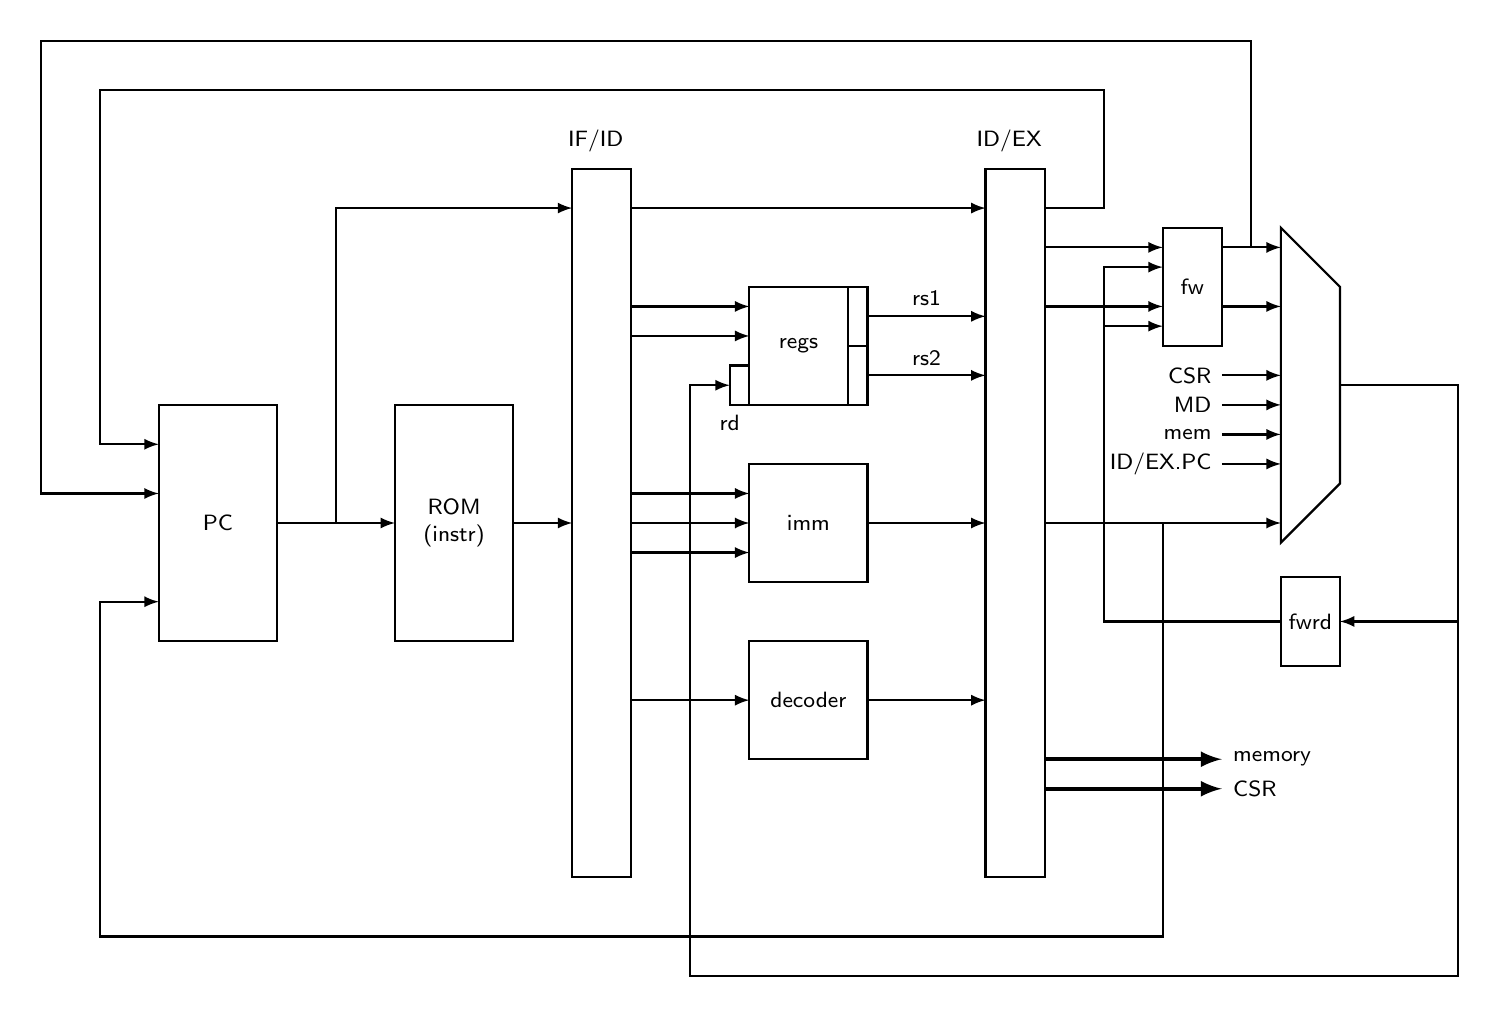
\begin{tikzpicture}[thick,font=\sffamily\footnotesize,>=latex,scale=.75,framed,background rectangle/.style={fill=none}]
% PC and Instruction ROM
\draw (0,0) rectangle node {PC} (2,-4);
\draw[-latex] (2,-2) -- (4,-2);
\draw (4,0) rectangle node[align=center] {ROM\\(instr)} (6,-4);
\draw (7,4) node[xshift=0.3cm,yshift=10pt] {IF/ID} rectangle node {} (8,-8);
\draw[-latex] (6,-2) -- (7,-2);
\draw[-latex] (3,-2) -- ++(0,5.333) -- ++(4,0);
\draw[-latex] (8,3.333) -- ++(6,0);
\draw[-latex] (15,3.333) -- ++(1,0) -- ++(0,2) -- ++(-17,0) -- ++(0,-6) --++(1,0);

% Registers, decoder and immediate generation
\draw (10,2) rectangle node {regs} (11.667,0);
\draw (11.667,1) rectangle ++(0.333,1);
\draw (11.667,0) rectangle ++(0.333,1);
\draw[-latex] (12,1.5) -- node[above] {rs1} ++(2,0);
\draw[-latex] (12,0.5) -- node[above] {rs2} ++(2,0);
\draw[-latex] (8,1.667) -- ++(2,0);
\draw[-latex] (8,1.667-.5) -- ++(2,0);
\draw[] (10-0.333, 0.667) rectangle ++(0.333,-0.667);

\draw[-latex] (8,-1.5) -- ++(2,0);
\draw[-latex] (8,-5.0) -- ++(2,0);
\draw[-latex] (8,-2.5) -- ++(2,0);
\draw[-latex] (12,-5) -- ++(2,0);
\draw[] (10,-1) rectangle node {imm} ++(2,-2);

\draw[] (10,-4) rectangle node[] {decoder} ++(2,-2);
\draw[-latex] (8,-2) -- ++(2,0);
\draw[-latex] (12,-2) -- ++(2,0);
 
% ID/EX
\draw (14,4) node[xshift=0.3cm,yshift=10pt] {ID/EX} rectangle node {} (15,-8);
\draw[] (15,-2) -- ++(2,0) coordinate (w) -- ++(0,0);
\draw[-latex] (w) -- ++(0,-7) -- ++(-18,0) -- ++(0,5.667) -- ++(1,0);
\draw (17,3) rectangle node{fw} ++(1,-2);
\draw[-latex] (15,2.667) -- ++(2,0);
\draw[-latex] (15,1.667) -- ++(2,0);

% ALU
\draw[] (19,3) -- ++(1,-1) -- ++(0,-3.333) -- ++(-1,-1.0) -- cycle; %++(0,3.333);
\draw[-latex] (17,-2.000) -- ++(2,0);
\draw[-latex] (18,2.667) -- ++(1,0);
\draw[-latex] (18,1.667) -- ++(1,0);
\draw[-latex] (18.5,2.667) -- ++(0,3.5) -- ++(-20.5,0) -- ++(0,-7.667) -- ++(2,0);
\draw[-latex] (18.0,0.5) node[left] {CSR} -- ++(1,0);
\draw[-latex] (18.0,0.0) node[left] {MD} -- ++(1,0);
\draw[-latex] (18.0,-0.5) node[left] {mem} -- ++(1,0);
\draw[-latex] (18.0,-1.0) node[left] {ID/EX.PC} -- ++(1,0);

% ALU out
\draw[-latex] (20,0.333) -- ++(2,0) -- ++(0,-4.0) coordinate (x) -- ++(-2,0);
\draw[] (20,-3+0.1667/2) rectangle node {fwrd} ++(-1,-1.5);

\draw[-latex] (19,-3.667) -- ++(-3,0) coordinate (z) -- ++(0,6) -- ++(1,0);
\draw[-latex] (16,1.333) -- ++(1,0);
%\draw[-latex,red] (z) -- ++(0,-8) -- ++(-18,0) -- ++(0,8) -- ++(2,0);

\draw[-latex] (x) -- ++(0,-6) -- ++(-13,0) coordinate (y) -- ++(0,10) -- ++(0.667,0) node[below,yshift=-7pt] {rd};

\draw[-latex,ultra thick] (15,-6) -- ++(3,0) node[right] {memory};
\draw[-latex,ultra thick] (15,-6.5) -- ++(3,0) node[right] {CSR};

\end{tikzpicture}
\caption{Overview of the RISC-V core. Not all connections are shown.}
\label{fig:blockdiagram}
\end{sidewaysfigure}

\subsection{Registers}
The register file consists of thirty-two 32-bit registers denoted by \texttt{x0} to \texttt{x31}. Internally, the registers use Big Endian format. Register \texttt{x0} (alias \texttt{zero}) is hardwired to all zeros. Writing this register has no effect. Reading this register returns all zero bits. Normally, the \texttt{x}-names are not used but may be handy when simulating the designs. Table~\ref{tab:registers} shows the names of the registers as they should be used.

A register can be written to, and two register can be selected for data and/or base address.

\begin{table}[!ht]
\centering
\caption{RISC-V registers and their purpose.}
\label{tab:registers}
\begin{tabular}{lllc}
Register & Name & Purpose & Saver \\
\midrule
\texttt{x0}      & \texttt{zero}   & Hard-wired zero                   & $-$ \\
\texttt{x1}      & \texttt{ra}     & Return address                    & Caller \\
\texttt{x2}      & \texttt{sp}     & Stack pointer                     & Callee \\
\texttt{x3}      & \texttt{gp}     & Global pointer                    & $-$ \\
\texttt{x4}      & \texttt{tp}     & Thread pointer                    & $-$ \\
\texttt{x5}      & \texttt{t0}     & Temporary/alternate link register & Caller \\
\texttt{x6-x7}   & \texttt{t1-t2}  & Temporaries                       & Caller \\
\texttt{x8}      & \texttt{s0/fp}  & Saved register/frame pointer      & Callee \\
\texttt{x9}      & \texttt{s1}     & Saved register                    & Callee \\
\texttt{x10-x11} & \texttt{a0-a1}  & Function arguments/return values  & Caller \\
\texttt{x12-x17} & \texttt{a2-a7}  & Function arguments                & Caller \\
\texttt{x18-x27} & \texttt{s2-s11} & Saved registers                   & Callee \\
\texttt{x28-x31} & \texttt{t3-t6}  & Temporaries                       & Caller
\end{tabular}
\end{table}

The register can optionally be put in ALM flip-flops. This increases the ALM count, but may have a positive effect in the clock speed.

\subsection{ALU}
\label{sec:alu}
The Arithmetic and Logic Unit (ALU) handles almost all computations on data. It can add, subtract, do logic operations such as AND, OR en XOR, can shift data left or right, and sign extend byte and half word data. Some operations require two registers, some only use one register. Some instructions use one register and immediate data. Furthermore the ALU is also used to determine if a conditional branch should be taken. Note that the RISC-V programmer's model does not incorporate status flags as some other architectures do. This requires some extra instructions when adding or subtracting double word (64-bit) data. This is handled by the C compiler. The ALU is also used to compute the return address from unconditional function calls (JAL and JALR instructions). The data is in Big Endian format. The ALU is the only building block that can write registers. The ALU does not compute multiplications and divisions, but merely passes on data from the MD unit.

Note that the computation of jump target addresses is handled by the Program Counter (PC) hardware.

\subsection{PC}
\label{sec:pc}
The Program Counter contains the address of the currently fetched instruction. The address is always on a 4-byte boundary although function calls and conditional jump (JAL, JALR en B$xx$ instructions) can be on non 4-byte boundaries (the C compiler will always create 4-bytes boundaries). The PC (or rather the VHDL description of the PC) handles the address calculations of jumps and branches taken. %Currently, the two lower bits of the PC are set to 0.

\subsection{Instruction Decoder}
\label{sec:instructiondecoder}
The instruction decoder decodes the instruction supplied by the ROM as pointed by the PC. An instruction is 4 bytes wide and in Little Endian order. The instruction decoder provides all control signals for the ALU, RAM, ROM, I/O, the PC, the Address Decoder, the CSR, the LIC the register file and the MD unit. %Some signals are directly wired to the memory.

\subsection{Control Unit}
The processor uses a twelve-state FSM, see Figure~\ref{fsmpipe}. Upon reset, the processor starts in state \lstinline|boot0|. In this state, the processor is executing a hardware no-operation, i.e.\@ no computations are performed, but register \lstinline|x0| (alias \lstinline|zero|) is written with all-zero bits. This is because onboard RAM-blocks (where the registers are placed), cannot have a reset signal. In state \lstinline|boot1| the processor performs a hardware no-operation (but the first instruction is being decoded). In the \lstinline|exec| state, the processor is executed decoded instructions. If a trap request is being asserted, the processor executes the trap initiate sequence (saving the PC, fetching the handler start address, pipeline is flushed). If a memory access is requested, the processor initiates the memory access sequence (state \lstinline|mem|). The processor waits in this state until the memory access is acknowledged. A jump (JAL, JALR) or a branch taken causes the processor to flush the pipeline and start fetching instruction from the target address (states \lstinline|flush| and \lstinline|flush2|). When the processor executes an integer multiply/divide instruction, the processor starts the MD sequence (states \lstinline|md| and \lstinline|md2|), and waits until the operation is completed. When the processor executes an \lstinline|mret| instruction, the processor executes the return sequence (fetching the saved PC, flushing the pipeline).

Note that a trap (interrupts and exceptions) can be initiated in the \lstinline|exec| state and has priority over the others signals. Note that a trap (exceptions only) can be initiated in the \lstinline|mem| state. In all other states, a trap can never be initiated.

\begin{figure}[!ht]
\centering
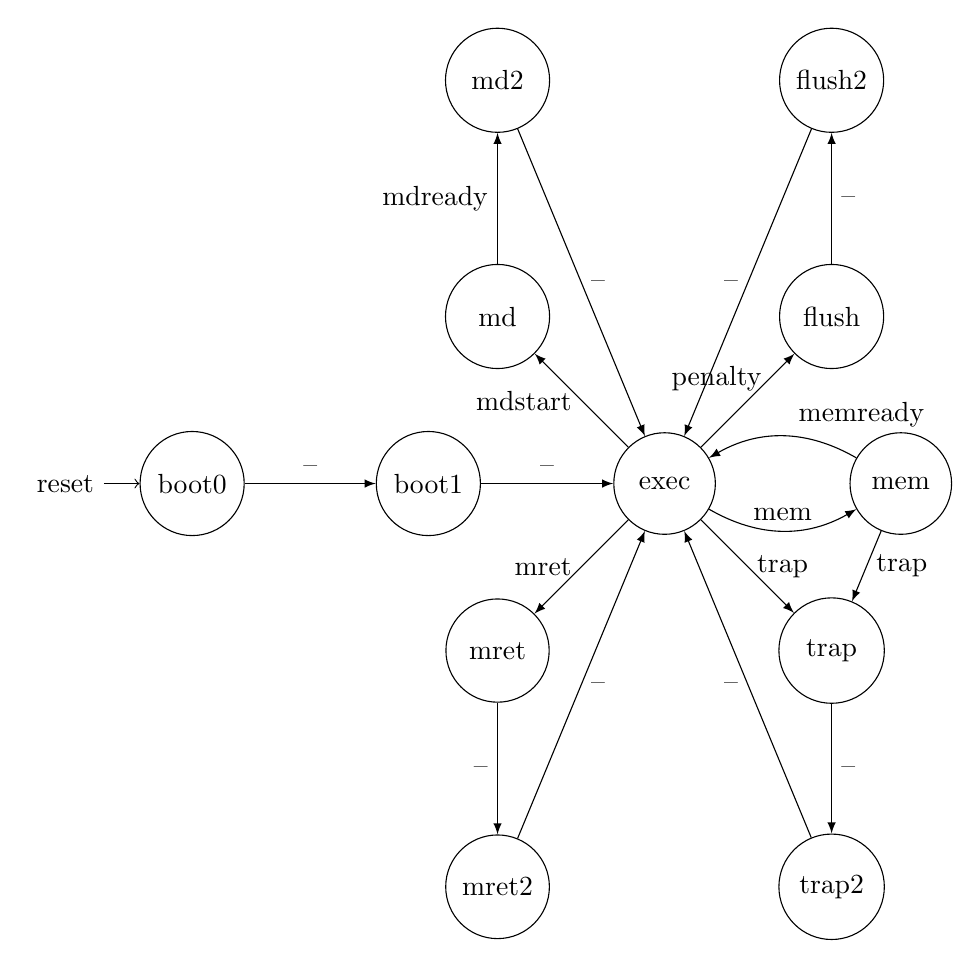
\begin{tikzpicture}[node distance=3cm, state/.style={circle, draw, minimum size=1cm,text width=1cm,align=center}]
\node[state,initial,initial text=reset] (boot0) {boot0};
\node[state,right of=boot0] (boot1) {boot1};
\node[state,right of=boot1] (exec) {exec};
\node[state,right of=exec] (mem) {mem};
\node[state,above left of=exec] (md) {md};
\node[state,above of=md] (md2) {md2};
\node[state,above right of=exec] (flush) {flush};
\node[state,above of=flush] (flush2) {flush2};
\node[state,below right of=exec] (trap) {trap};
\node[state,below of=trap] (trap2) {trap2};
\node[state,below left of=exec] (mret) {mret};
\node[state,below of=mret] (mret2) {mret2};

\path[-latex] (boot0) edge node[above] {--} (boot1)
              (boot1) edge node[above] {--} (exec)
              (exec) edge [bend right] node[above] {mem} (mem)
              (mem) edge [bend right] node[above,xshift=1cm] {memready} (exec)
              (mem) edge node[right] {trap} (trap)
              (exec) edge node[left] {mdstart} (md)
              (md) edge node[left] {mdready} (md2)
              (md2) edge node[right] {--} (exec)
              (exec) edge node[above left,xshift=0.3cm] {penalty} (flush)
              (flush) edge node[right] {--} (flush2)
              (flush2) edge node[left] {--} (exec)
              (exec) edge node[right,] {trap} (trap)
              (trap) edge node[right] {--} (trap2)
              (trap2) edge node[left] {--} (exec)
              (exec) edge node[left] {mret} (mret)
              (mret) edge node[left] {--} (mret2)
              (mret2) edge node[right] {--} (exec)
;
%\node at (0,-4) {\small * trap initiated by hardware or software.};
\end{tikzpicture}
\caption{FSM of the instruction flow of the processor.}
\label{fsmpipe}
\end{figure}

The PC points to +8 of the currently executing instruction, in a sequential instruction stream. If a jump or branch taken occurs, the FSM inserts a penalty because the PC has to be loaded with the correct value and a new instruction must be fetched (Figure~\ref{fsmpipeseqstartup}). Reading RAM, ROM and I/O requires three clock cycles (Figure~\ref{fsmpipeseqwait}), a write requires two clock cycles. When a multiply, divide or remainder instruction is encountered, the FSM enters the \texttt{md} state and waits for the md-unit to complete (32+2 or 16+2 clock cycles). Note that \lstinline|penalty|, \lstinline|mem|, \lstinline|mdstart| and \lstinline|mret| cannot occur at the same time.

\begin{figure}[!ht]
\centering
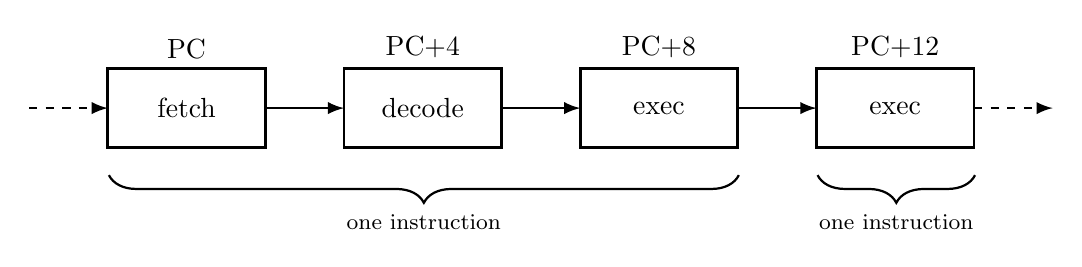
\begin{tikzpicture}[node distance=2cm, line width=1pt]
\draw[-latex,dashed] (-1,-0.5) -- ++(1,0);

\draw (0,0) rectangle node [] {fetch} ++(2,-1);
\node at (1,0) [above] {PC};
\draw[-latex] (2,-0.5) -- ++(1,0);

\draw (3,0) rectangle node [] {decode} ++(2,-1);
\node at (4,0) [above] {PC+4};
\draw[-latex] (5,-0.5) -- ++(1,0);

\draw (6,0) rectangle node [] {exec} ++(2,-1);
\node at (7,0) [above] {PC+8};
\draw[-latex] (8,-0.5) -- ++(1,0);

\draw (9,0) rectangle node [] {exec} ++(2,-1);
\node at (10,0) [above] {PC+12};
\draw[-latex,dashed] (11,-0.5) -- ++(1,0);

\draw [thick,decorate,decoration={brace,amplitude=10pt,mirror},xshift=0.4pt,yshift=-10pt](0,-1) -- (8,-1) node[black,midway,yshift=-0.6cm] {\footnotesize one instruction};
\draw [thick,decorate,decoration={brace,amplitude=10pt,mirror},xshift=0.4pt,yshift=-10pt](9,-1) -- (11,-1) node[black,midway,yshift=-0.6cm] {\footnotesize one instruction};
\end{tikzpicture}
\caption{State sequence for start up/penalty with instruction execution (no wait state).}
\label{fsmpipeseqstartup}
\end{figure}

\begin{figure}[!ht]
\centering
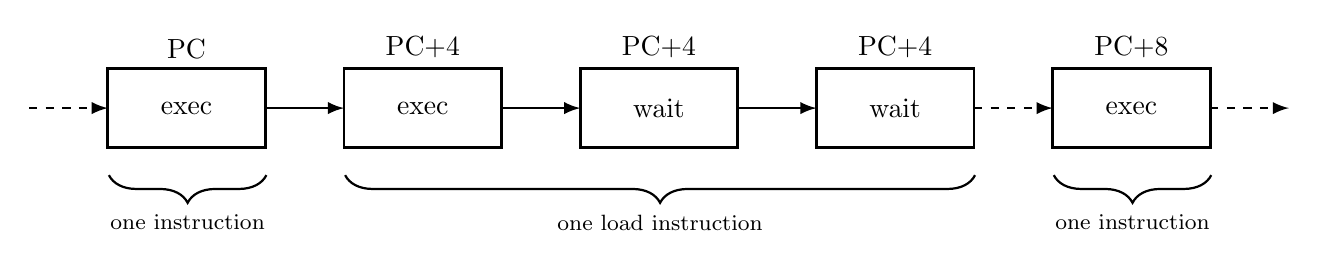
\begin{tikzpicture}[node distance=2cm, line width=1pt]
\draw[-latex,dashed] (-1,-0.5) -- ++(1,0);

\draw (0,0) rectangle node [] {exec} ++(2,-1);
\node at (1,0) [above] {PC};
\draw[-latex] (2,-0.5) -- ++(1,0);

\draw (3,0) rectangle node [] {exec} ++(2,-1);
\node at (4,0) [above] {PC+4};
\draw[-latex] (5,-0.5) -- ++(1,0);

\draw (6,0) rectangle node [] {wait} ++(2,-1);
\node at (7,0) [above] {PC+4};
\draw[-latex] (8,-0.5) -- ++(1,0);

\draw (9,0) rectangle node [] {wait} ++(2,-1);
\node at (10,0) [above] {PC+4};
\draw[-latex,dashed] (11,-0.5) -- ++(1,0);

\draw (12,0) rectangle node [] {exec} ++(2,-1);
\node at (13,0) [above] {PC+8};
\draw[-latex,dashed] (14,-0.5) -- ++(1,0);

\draw [thick,decorate,decoration={brace,amplitude=10pt,mirror},xshift=0.4pt,yshift=-10pt](0,-1) -- (2,-1) node[black,midway,yshift=-0.6cm] {\footnotesize one instruction};
\draw [thick,decorate,decoration={brace,amplitude=10pt,mirror},xshift=0.4pt,yshift=-10pt](3,-1) -- (11,-1) node[black,midway,yshift=-0.6cm] {\footnotesize one load instruction};
\draw [thick,decorate,decoration={brace,amplitude=10pt,mirror},xshift=0.4pt,yshift=-10pt](12,-1) -- (14,-1) node[black,midway,yshift=-0.6cm] {\footnotesize one instruction};
\end{tikzpicture}
\caption{State sequence for instruction execution (wait state).}
\label{fsmpipeseqwait}
\end{figure}

\subsection{Trap handling}
When an interrupt occurs, the FSM enters the \texttt{trap} state for fetching the trap vector. An interrupt can occur any time and is called asynchronous. When an interrupt occurs,
the current instruction is discarded and must be restarted after return. After fetching the trap handler, new instructions are fetched and the instruction pipeline is flushed.

Exceptions are synchronous to the executing of instructions. When an exception occurs, the current instruction is discarded and must be restarted after return. Exceptions to this are the ECALL and EBREAK instructions. These instructions do cause a trap, but are not restarted, so the next instruction must be fetched after return. This has to be handled in software by the trap handler. 

Note that interrupts are only served in the \lstinline|exec| state.
An ongoing memory access can only be interrupted by an exceptions (\lstinline|mem| state). An ongoing hardware multiply/divide operation is \emph{not} interrupted, the operation completes (and writes back the result in a register).

When a trap request is asserted, the trap vector is loaded in the next clock cycle. Then, in the second clock cycle, the instruction is fetched and in the third clock cycle the instruction is decoded and in the fourth cycle the instruction is executed. On return from a trap handler, the original contents of the PC is fetched from the CSR and then instructions are fetched. A return flushes the pipeline. Also see Section~\ref{sec:traphandling}.

The following exceptions are implemented:
\begin{itemize}
\item ECALL -- M-mode only
\item EBREAK -- break to debugger
\item Load access fault -- reading unimplemented memory
\item Store access fault -- writing unimplemented memeory
\item Load address misaligned -- not natural aligned for halfword and word
\item Store address misaligned -- not natural aligned for halfword and word
\item Illegal instruction -- instruction is not valid
\item Instruction access fault -- reading unimplemented memory
\item Instruction address misaligned -- not on a 4-byte boundary
\end{itemize}

The \lstinline|mtval| CSR is written with offending memory address for load/store access/misaligned fault. For the remaining exceptions \lstinline|mtval| is set to all-zero bits.

\subsection{Address Decoder and Data Router}
\label{sec:addressdecoderanddatarouter}
The Address Decoder and Data Router routes reads and writes to the ROM, bootloader ROM (only reads), RAM and the I/O. The processor uses a 32-bit linear address space for ROM, boot ROM, RAM and I/O. The address space is divided in 16 parts of 256 MB each. In the default setting, ROM starts at address 0x00000000 and the length is 64 kB. The bootloader ROM starts at address 0x10000000 and the length is 4 kB. Unused ROM addresses return 0x0000000. The RAM starts at address 0x20000000 and length is 32 kB. The I/O starts at address 0xF0000000 and the length is 16 kB by default.

When data is read, the data is collected from the accessed memory and put on an internal bus to the ALU. The ALU can perform sign extension (byte and half word accesses) if needed. Please note that reading data from the ROM, bootloader ROM, RAM and I/O requires three clock cycles. Writing requires two clock cycles.

Note that instructions can only be fetched from ROM and boot ROM.

\subsection{Instruction Router}
The Instruction Router routes instructions from the ROM and the boot ROM. If the boot ROM is disabled, the synthesizer will remove access to boot ROM.

\subsection{Control and Status registers}
The RISC-V specification describes a set of 4096 control and status register in a separate address space. CSR operations require one clock cycle. Basic event counters are implemented:

\begin{itemize}
\item \lstinline|cycle| and \lstinline|cycleh| -- these 32-bit registers form a 64-bit value that contains the counted clock cycles since the last reset.
\item \lstinline|time| and \lstinline|timeh| -- these registers shadow the contents of the \lstinline|MTIME| and \lstinline|MTIMEH| registers from the I/O.
\item \lstinline|instret| and \lstinline|instreth| -- these 32-bit registers form a 64-bit value that contains the counted retired instructions since the last reset.
\end{itemize}

Note that these registers are read-only. Writes are ignored. 

Generic registers:

\begin{itemize}
\item \lstinline|mvendorid| -- this register is hardwired to all zero bits.
\item \lstinline|marchid| -- this register is hardwired to all zero bits.
\item \lstinline|mimpid| -- this register is hardwired to the current version of the hardware.
\item \lstinline|mhartid| -- this register is hardwired to all zero bits.
\item \lstinline|mconfigptr| -- this register is hardwired to all zero bits.
\item \lstinline|misa| -- hardwired to value 0x40001100, indicating 32-bit processing, RV32I base ISA and Integer Multiply/Divide extension, or hardwired to 0x40001010 for E extension. If the MD unit is excluded from the design, bit 12 of \lstinline|misa| is 0.
\end{itemize}

For trap handling, the following registers are implemented:

\begin{itemize}
\item \lstinline|mstatus| -- the only implemented bits are \lstinline|MIE|, \lstinline|MPIE| and \lstinline|MPP|, all other bits are hardwired zero.
\item \lstinline|mie| -- for the lower 16 bits, only \lstinline|MTIE| is implemented, all other bits are hardwired zero.
\item \lstinline|mtvec| -- contains the trap handler (vector) address, can be used in direct and vectored mode, and bit 1 is always 0.
\item \lstinline|mstatush| -- this register is hardwired to all zero bits.
\item \lstinline|mscratch| -- currently not used, but can be used by software trap handlers.
\item \lstinline|mepc| -- contains the PC at point of trap of the \emph{currently} executing instruction.
\item \lstinline|mcause| -- contains the cause of the trap as set forward in ``The RISC-V Instruction Set Manual, Volume II: Privileged Architecture''. For local interrupts, additional codes are used.
\item \lstinline|mtval| -- contains the address on the address bus when a trap occurs, or all-zero bits if not relevant.
\item \lstinline|mip| -- contains the pending interrupts. For the lower 16 bits, only \lstinline|MTIP| is implemented. The upper 16 bits are used for local interrupts. This register is read-only.
%\item \lstinline|mconfigptr| -- this register is hardwired to all zero bits.
\item \lstinline|mcountinhibit| -- this register has bit 2 (\lstinline|minstret|) and bit 0 (\lstinline|mcycle|) implemented.
\end{itemize}

Custom CSR:

\begin{itemize}
\item \lstinline|mxhw| -- this custom CSR with address \lstinline|0xfc0| is read-only and reflects the hardware properties of the synthesized processor.
\item \lstinline|mxspeed| -- this custom CSR with address \lstinline|0xfc1| is read-only and contains the system frequency in Hz of the synthesized processor (see Section~\ref{sec:hardware}).
\end{itemize}
%The \lstinline|mcounteren| register is not implemented, because U-mode is not implemented. The \lstinline|menvcfg| and \lstinline|menvcfgh| are not implemented, because only M-mode is implemented.

Writing read-only registers causes an illegal instruction trap. Accessing a non-existent register causes an illegal instruction trap. The trap handler (vector) address must be loaded by software at boot time (normally done in \lstinline|main|). Both direct and vectored mode are supported. In direct mode all traps redirect to a single trap handler that has to handle both interrupts and exceptions. The most significant bit of \lstinline|mcause| is 1 when a trap occurred from an interrupt. In vectored mode, the addresses of \emph{interrupt handlers} are loaded from a jump table. Exceptions are redirected to a single handler. Note that the address of the jump table must be on a 4-byte boundary, and bit 0 of \lstinline|mtvec| must be set to 1 for vectored mode.


\subsection{Local Interrupt Controller}
The Local Interrupt Controller is responsible for selecting which trap request must be serviced by the core. Interrupts have higher priority than exceptions. The state of the serviced trap is visible in the CSR.

The LIC can handle 16 local interrupts (numbered 16 to 31) and the Machine mode external timer interrupt (numbered 7). Other standard RISC-V interrupts (numbered 0 to 6 and 8 to 15) are not available. SPI1 has the highest priority, followed (currently) by the I2C1, I2C2, UART1, TIMER2, TIMER1, EXTI external input interrupt and external system timer interrupts. We reserve number 31 for the NMI, if ever implemented.

Exceptions are handled as set forward in Table 3.7 of ``The RISC-V Instruction Set Manual, Volume II: Privileged Architecture'': instruction access fault, instruction address misaligned, ECALL (M mode only), EBREAK, load/store address misaligned, load/store access fault. Note that ECALL and EBREAK are user instructions and can be interrupted by an interrupt (i.e. when the ECALL or EBREAK instruction is executing).


\subsection{Multiply/Divide Unit}
The processor is equipped with a hardware integer multiply/divide unit. All multiply/divide instructions are supported (\lstinline|MUL|, \lstinline|MULH|, \lstinline|MULHSU|, \lstinline|MULHU|, \lstinline|DIV|, \lstinline|DIVU|, \lstinline|REM|, \lstinline|REMU|) and the result is fed to the ALU. A multiplication takes three clock cycles (one clock-in, one multiply, one clock-out). For division, two versions are available. By default, the divider needs 18 clocks (one clock-in, 16 divide, one clock-out) for a division using a poor man's radix-4 division unit. As an alternative, a simple radix-2 division unit can be selected taking 34 clock cycles (one clock-in, 32 divide, one clock-out) to do the division.  Thus, the radix-4 divider unit is faster, but needs more cells. The radix-2 divider unit is slower, but needs less cells. You have to enable the M-standard support in the compiler. The multiplier uses special DSP units in the Cyclone V. Most regular FPGAs have onboard multipliers. Note that when executing an operation, the pipeline is stalled. Note that a trap request is postponed until the operation is completed and the result is saved in the register file. Selecting the radix-4 division has a minimum impact on the clock speed.


\subsection{Stack pointer}
The stack pointer is fully implemented although the ISA does not provide pushes and pops. The stack pointer is used to allocate local variables and is updated with each allocation and deallocation. As usual, the stack grows downwards (to lower addresses) on allocations and upwards (to higher addresses) on deallocations. Therefore the stack pointer is set to the highest RAM address + 1 on boot (which is 0x20008000 by default). The ISA postulates that the stack is aligned on 16-byte boundaries for the I standard.


\subsection{ROM}
\label{sec:rom}
The ROM consists of bytes and is only word addressable for instructions. The ROM is byte, half word and word addressable when reading constant data. Half word and word entries are in Litte Endian format. When reading data from the ROM, half word accesses must be on 2-byte boundaries and word accesses must be on 4-byte boundaries. This simplifies the decoding circuitry. The ROM returns undefined data if an access is not aligned and will generate an exception. The processor instantiates the ROM in onboard RAM. Rearranging half word and word data accesses in Big Endian format is handled by the ROM decoding unit. Reading ROM (as data) requires three cycles.  This is automatically handled by the processor. The pipeline is stalled for two clock cycles when reading from ROM (data). Reading instructions requires two clock cycles.

When the bootloader hardware is installed, the ROM is writable as words only. Although this write option is reserved for the bootloader,  a user program can manipulate the ROM. A write requires one or two clock cycles, depending on the VHDL generic \lstinline|HAVE_FAST_STORE|. See Section~\ref{sec:customize}.

Note: the Cyclone V 5CEBA4F23C7 has 3,153,920 bits of onboard RAM available. Because of the 32-bit entries a maximum of 2,097,152 (65536 x 32) bits can be instantiated. This is equivalent to 262,144 bytes.

Note: instructions can only be fetched from the ROM and bootloader ROM. Note: when the bootloader is synthesized in the FPGA, the ROM may also be written with 32-bit data on 4-byte boundaries.

\subsection{Bootloader ROM}
\label{sec:bootloaderrom}
The bootloader ROM contains a small program to upload S-record files in the ROM. The bootloader ROM cannot be written by an upload. Besides that, the bootloader contains a simple monitor program. The bootloader ROM is places in onboard immutable RAM blocks. See Section~\ref{sec:bootloader}. The bootloader may be excluded from synthesis.

\subsection{RAM}
\label{sec:ram}
The RAM consists of bytes and is byte, half word and word addressable. Half word and word entries are in Little Endian format. The RAM itself is made up of word (i.e. 32-bit) entries and is instantiated with onboard RAM blocks. Due to this fact, half word accesses are only permitted on 2-byte boundaries and word accesses are only permitted on 4-byte boundaries. The RAM returns undefined data if an access is not aligned. Writes will not take place if an access is unaligned. This simplifies the decoding circuitry. Unaligned accesses cause an exception. For the Cyclone V a maximum of 65536 words of RAM can be instantiated. Rearranging half word and word data accesses in Big Endian format is handled by the RAM decoding unit. The RAM cannot be used for program data.

Note: the Cyclone V 5CEBA4F23C7 has 3,153,920 bits of onboard RAM available. Because of the 32-bit entries a maximum of 2,097,152 (65536 x 32) bits can be instantiated. This is equivalent to 262,144 bytes.

Reading the RAM (byte, half word, word) requires three clock cycles. A write requires one or two clock cycles, depending on the VHDL generic \lstinline|HAVE_FAST_STORE|. See Section~\ref{sec:customize}.

\subsection{I/O}
\label{sec/io}
Currently, the I/O consists of one 32-bit data input and one 32-bit data output, a simple UART with interrupts, a simple timer with interrupt, a more elaborate timer with interrupt, two minimal I\textsuperscript{2}C peripherals with interrupt, a general purpose SPI peripheral with interrupt, a dedicated SPI peripheral for SD card access and the TIME and TIMEH memory mapped time registers with interrupt. Note that the I/O can only be accessed as words and the addresses must be on 4-byte boundaries. If not on a 4-byte boundaries or not word size reads/writes, reads return undefined data whereas writes will not write data. Unaligned accesses cause an exception. A read requires three clock cycles, a write requires one or two clock cycles, depending on the VHDL generic \lstinline|HAVE_FAST_STORE| (s)ee Section~\ref{sec:customize}). Note that not all I/O addresses are used.

GPIOA has separate inputs and output, both 32 bits. This is because some FPGAs/synthesizers don't allow buried tri-state signals, i.e.\@ the tri-state action must be done in the top level entity. Because of that, there is no data direction register. Currently the inputs come from the slide switches and the push buttons. Note that KEY4 a.k.a.\@ FPGA\_RESET is connected to the reset of the processor. The outputs are connected to the 10 red leds and to the two least significant 7-segment displays. Also two output pins are connected to facilitate SPI software generated NSS signals. The GPIOA module is equipped with a pin input edge detector generating an interrupt is a rising and/or falling edge is detected.

UART1 can transmit and receive data at 7, 8 or 9 bits, no/even/odd parity and 1 or 2 stop bits. Tested speeds are 9600 bps, 115200 bps and 230400 bps. Several status flags are implemented to guide transmission. Receive and transmitted character (local) interrupts are provided (one vector). These interrupt requests must be negated by software. UART1 does not provide hardware flow control.

TIMER1 has a 32-bit count register and increments on every clock cycle. It does not have a prescaler. It counts up to compare match T register, after which is will be loaded with 0 again. A compare match (local) interrupt is provided (one vector). Whenever the timer count register is greater than or equal to the compare match T register, an interrupt request is asserted in the next clock cycle. The interrupt request has to be negated by software. A value of 0 in the compare match T register is valid: the counter does not count, but the compare match (local) interrupt is asserted.

TIMER2 has a 16-bit count register and a 16-bit prescaler, and increments on every clock cycle. The counter can be used to generate signals (Output Compare/PWM) or detect incoming signal edges (Input Capture). When in output mode. the timer counts up to compare match T register, after which is will be loaded with 0 again. Compare match (local) interrupts are provided (one vector). Whenever the timer count register is greater than or equal to the compare match T register, an interrupt request is asserted. The interrupt request has to be negated by software. The timer provides three Channels with compare registers (A, B, C). Whenever the timer count register is greater than or equal to a compare register (A, B, C) the respective interrupt request is asserted. The interrupt requests have to be negated by software. A value of 0 in the compare match T register is valid: the counter does not count, but the compare match T (local) interrupt is asserted and the compare match interrupts (A, B, C) are asserted whenever the respective compare match register is 0. The prescaler is always preloaded: if the timer is off, the shadow prescaler register is directly written, if the timer is running, the preload register is written and the shadow register is updated at the the next CMPT match. The CMPT/A/B/C registers may optionally use a preload register. If preload is off, the shadow registers are directly written, if preload is on, the preload registers are written and the shadow registers are updated at the next CMPT match. In Input Compare mode, the Channels A, B and C can be selected to trigger on a positive or negative edge. When an edge is detected, the current value of CNTR is copied to the accompanying CMP$x$ register and the accompanying interrupt flag is asserted. Note that Channel T cannot be used for PWM and input capture. The input capture circuits use a two-stage synchronizer. 

I2C1 is a minimal I\textsuperscript{2}C controller peripheral (master-only). It cannot react to clock stretching and lost arbitration, so only modern targets (slaves) can be connected in a one-master-only system. Both Standard mode (Sm) with a transmission speed of up to 100 kbps and Fast mode (Fm) with a transmission speed up to 400 kbps are implemented. Before sending the address byte, the send-start bit must be set and a START condition is send to the target when the address is written to the I2C1 data register. Before sending or receiving the last data byte, the send-stop bit must be set and a STOP condition is send to the target after the byte is send or received by the controller. The last byte received will not be acknowledged by the controller. When receiving intermediate bytes, the controller must acknowledge the reception with an ACK. This is controlled by the MACK bit in the control register. Sending a byte is straightforward: just write the byte to the data register. When receiving a byte, a dummy byte (data value of 0xff) must be send to the target. This way, the processor can create a pause in the transmission if needed. Note that the SCL line is kept low between byte transmissions. The baud rate prescaler must be loaded with the number of system clock cycles of \textbf{one-half} bit time minus~1 for Standard mode and \textbf{one-third} bit time minus~1 for Fast mode. Note that the prescaler is part of the control register CTRL and its value must be preserved when setting or clearing other bits. The SCL and SDA inputs are synchronized to the system clock using two 2-bit shift registers.

I2C2 is exact copy of I2C1, except that it doesn't have an interrupt.

SPI1 is a full-fledged SPI master. It can transfer 8-bit, 16-bit, 24-bit and 32-bit data in one SPI cycle. It incorporates a programmable prescaler (from /2 to /256 in powers of 2) and all four phases of clock polarity (CPOL) and phase polarity (CPHA), hardware NSS (Slave Select, active low) and programmable Slave Select setup and hold time. It is possible to use a GPIO pin to use software-controlled NSS. Currently, the MISO is not synchronized to the system clock.

SPI2 is a simple SPI master dedicated for the micro SC card reader. It can transfer 8-bit, 16-bit, 24-bit and 32-bit data in one SPI cycle. It does not have an hardware NSS signal and no interrupt capability. A single I/O pin is needed for NSS. Currently, the MISO is not synchronized to the system clock.

The I/O incorporates memory mapped TIMEH:TIME and TIMECMPH:TIMECMP registers. Whenever TIMEH:TIME (as viewed as a 64-bit register) is greater than or equal to TIMECMPH:TIMECMP (as viewed as a 64-bit register) an interrupt request is asserted. The interrupt request is negated if TIMEH:TIME is less than TIMECMPH:TIMECMP. This has to be handled by software. Currently the TIMEH and TIME registers cannot be written. Note that TIMEH:TIME counts the number of microseconds since last reset. The toolchain expects this since \lstinline|clock()| and \lstinline|gettimeofday()| depend on this value. As such, the system clock frequency must be a integer multiple of 1\,MHz. Note that TIMEH:TIME is writable by software.

\subsection{Implemented instructions}
For the processor, all RV32IM Unprivileged instructions are implemented but the FENCE instruction act as a no-operation (NOP). ECALL and EBREAK are supported and execute an exception. Also, the Zicsr instructions are implemented. From the Privileged instruction, MRET is used to return from an exception or an interrupt. WFI is not implemented and acts as a no-operation (NOP). FENCE and FENCE.I are not implemented and act as a NOP.

\section{The FPGA}
For this project, we use the Cyclone V FPGA from Intel (formerly Altera). See \url{https://www.intel.com/content/www/us/en/products/details/fpga/cyclone/v.html}.
The used Cyclone V is the 5CEBA4F23C7 which has 18480 ALMs available. It has 3080 kb of onboard RAM bits available which are used for RAM, ROM, (possibly) bootloader ROM and (possibly) the registers. Depending on the program and used resources, the compiled RISC-V processor uses about 2900 ALMs (about 16\,\%) and 1,378,304 bits of internal memory (44\,\%). The clock frequency is approximately 80\,MHz, which is sufficient for all program examples. Note that the DE0-CV board has a onboard clock generator with a frequency of 50\,MHz, so a PLL is needed to get a frequency of 80\,MHz. This FPGA is mounted on a Terasic DE0-CV board (see Figure~\ref{fig:image-de0-cv}). The board has 10 switches, 4 push buttons, 1 reset push button, 10 leds, and 6 seven-segment displays. It also has two 2x20-pin headers to connect off-board devices. See \url{http://www.terasic.com.tw/cgi-bin/page/archive.pl?Language=English&No=921}. For downloading the bitstream file, the onboard USB-Blaster is used.

\begin{figure}[!ht]
\centering
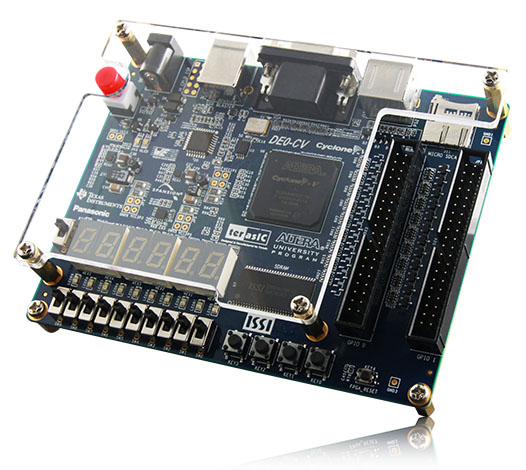
\includegraphics[scale=0.45]{images/image-de0-cv}
\caption{The DE0-CV board.}
\label{fig:image-de0-cv}
\end{figure}

Disabling the bootloader saves one copy of the ROM and the bootloader ROM. Then the used RAM is 786,432 bits (25\,\%). Disabling registers in RAM saves 2048 bits, but increases the ALM count. You may see some warnings from the synthesizer.

It is possible to add the Quartus' Signal Tap (embedded) Logic Analyzer. Follow the instructions on \url{https://people.ece.cornell.edu/land/courses/ece5760/Quartus/Signal_tap.html}. Note that the Signal Tap uses onboard memory.

To find the best compilation result for speed and/or area, we have to tweak the compiler setting for the synthesizer and the fitter. Best is to do a design space exploration, and randomize the seed. Tweaking the seed may show a difference of 5\,MHz on the clock speed.

Table~\ref{tab:util} gives some estimates on the design. In all cases, the seed is set to 1 and the optimization is set to balanced. The total amount of ALMs is 18480. The total amount of RAM bits is 3153920.

\begin{table}[!ht]
\caption{FPGA resource utilization for the DE0-CV board (Slow 1100mV 85C model).}
\label{tab:util}
\centering
\begin{tabular}{lllll}
\toprule
     & \begin{tabular}[c]{@{}l@{}}no boot\\ no reg in ram\end{tabular} & \begin{tabular}[c]{@{}l@{}}no boot\\ reg in ram\end{tabular} & \begin{tabular}[c]{@{}l@{}}boot\\ no reg in ram\end{tabular} & \begin{tabular}[c]{@{}l@{}}boot\\ reg in ram\end{tabular} \\ \midrule
Freq & 89.99   & 82.07   & 86.66     & 91.10     \\
ALM  & 3531    & 2893    & 3528      & 2911      \\
FF   & 3471    & 2393    & 3515      & 2390      \\
RAM  & 786,432 & 788,480 & 1,376,256 & 1,378,304 \\ \bottomrule
\end{tabular}
\end{table}

As you can see, there's a big difference is maximum frequency. Please select different seed values in the options of the synthesizer. Also disabling the Zba extension and unused peripherals may increase the maximum frequency and lowers the ALM and register count.

\section{Processor hardware}
\label{sec:hardware}
The processor hardware is composed of the following VHDL files:

\begin{itemize}
\item \lstinline|processor_common.vhd| -- Common types and constants.
\item \lstinline|address_decode.vhd| -- The address decoder and data router to the memory \item \lstinline|core.vhd| -- The core contains the PC, the registers, the ALU, the MD unit, the control state machine, the memory interface, the CSR and the LIC.
\item \lstinline|instr_router.vhd| -- Description of the instruction router.
\item \lstinline|rom.vhd| -- Description of the ROM. Will be placed in onboard, initialized RAM blocks. 
\item \lstinline|rom_image.vhd| -- Description of the ROM contents.
\item \lstinline|bootloader.vhd| -- Description of the bootloader ROM. The bootloader program will be placed in onboard, initialized RAM blocks. 
\item \lstinline|ram.vhd| -- Description of the RAM. Will be placed in onboard, uninitialized RAM blocks. 
\item \lstinline|io.vhd| -- Description of the I/O. It contains a 32-bit input register, a 32-bit output register, an UART, I2C, SPI, timers and the TIME and TIMECMP memory mapped registers.
\item \lstinline|riscv.vhd| -- Top-level description of the processor. Connects all the building blocks to a viable processor.
\item \lstinline|riscv.sdc| -- Constraints file. Sets the target clock frequency.
\item \lstinline|tb_riscv.vhd| -- VHDL testbench to simulate the design.
\item \lstinline|tb_riscv.do| -- QuestaSim/Modelsim command script.
\end{itemize}

%In the file \lstinline|processor_common.vhd|, a number of constant parameters are available:
%\begin{itemize}
%\item \lstinline|SYSTEM_FREQUENCY| -- Set to 50 MHz. Change this to suit the system clock frequency, for example when using a PLL.
%\item \lstinline|CLOCK_FREQUENCY| -- Set to 1 MHz. Used to calibrate the internal clock. The compiler assumes 1 MHz and some library functions depend on it. Used for measuring time in microseconds.
%\item \lstinline|NUMBER_OF_REGISTERS| -- Set to 32 for I standard. Set to 16 for E standard. You need to supply the correct architecture and ABI.
%\item \lstinline|HAVE_MULDIV| -- Set to TRUE, the MD unit is included. Set to FALSE to exclude MD unit. If set to false, you must not specify the hardware multiply/divide options while compiling software, i.e.\@ multiply and division occur in software.
%\item \lstinline|FAST_DIVIDE| -- Set to TRUE to use the radix-4 divider. Set to FALSE to use the radix-2 divider.
%\item \lstinline|VECTORED_MTVEC| -- Set to TRUE to provide vectored interrupts. You still have to set bit 0 to 1 in \lstinline|mtvec| CSR. You can still use direct mode. Set to FALSE to only use direct interrupts.
%\item \lstinline|MSTATUS_MIE_DISABLES_INTERRUPTS| -- Set to TRUE to only disable interrupts when \lstinline|mstatus.MIE| is 0. Set to FALSE to disable all traps (so including exceptions and when \lstinline|mstatus.MIE| is 0). This option can be used in simulations.
%\item \lstinline|HAVE_BOOTLOADER_ROM| -- Set to TRUE to provide the bootloader ROM and the PC is set to the start of the bootloader. Set to FALSE to disable the bootloader ROM and the PC is set to the start of the ROM. Disabling the bootloader reduces the RAM block count considerably.
%\item \lstinline|HAVE_REGISTERS_IN_RAM| -- Set to TRUE to place the registers in onboard RAM blocks. This lowers the ALM count drastically, but may have an impact on the system frequency. Set to FALSE to place the registers in ALM flip-flops.
%\item \lstinline|HAVE_UART1| -- Set to TRUE to include UART1 hardware. Set to FALSE to remove UART1 hardware.
%%\item \lstinline|HAVE_UART2| -- Set to TRUE to include UART2 hardware. Set to FALSE to remove UART2 hardware.
%\item \lstinline|HAVE_I2C1| -- Set to TRUE to include IC21 hardware. Set to FALSE to remove I2C1 hardware.
%\item \lstinline|HAVE_SPI1| -- Set to TRUE to include SPI1 hardware. Set to FALSE to remove SPI1 hardware.
%\item \lstinline|HAVE_SPI2| -- Set to TRUE to include SPI2 hardware. Set to FALSE to remove SPI2 hardware.
%\item \lstinline|HAVE_TIMER1| -- Set to TRUE to include TIMER1 hardware. Set to FALSE to remove TIMER1 hardware.
%\item \lstinline|HAVE_TIMER2| -- Set to TRUE to include TIMER2 hardware. Set to FALSE to remove TIMER2 hardware.
%\end{itemize}
%
%Note: GPIOA and the external timer (TIME et al.) are always included.

The entity of the top level (\lstinline|riscv.vhd|) is shown in the listing below.

\lstinputlisting[language=VHDL,breaklines=false]{code/riscv.vhd}

\subsection{Pin assignments}
The pin assignments for the DE0-CV board are as follows (Table~\ref{tab:pins}). Note that not all signals are assigned to a pin, in which case the fitter will assign a suitable pin.

\begin{longtable}{lll}
\caption{Pin assignments for the DE0-CV board.}
\label{tab:pins}\\
\toprule
\textbf{Signal} & \textbf{Pin Name} & \textbf{Board name, comments} \\
\midrule
\endfirsthead
\multicolumn{3}{c}%
{\textit{Continued from previous page}} \\
\toprule
\textbf{Signal} & \textbf{Pin Name} & \textbf{Board name, comments} \\
\midrule
\endhead
\bottomrule
\multicolumn{3}{r}{\textit{Continued on next page}} \\
\endfoot
\bottomrule
\endlastfoot
%\toprule
clk       & M9       & CLOCK\_50, System clock\\
areset    & P22      & FPGA\_RESET, active low reset\\
gpioapin[31]  & $-$      & Fitter assigned \\
gpioapin[30]  & $-$      & Fitter assigned \\
gpioapin[29]  & $-$      & Fitter assigned \\
gpioapin[28]  & $-$      & Fitter assigned \\
gpioapin[27]  & $-$      & Fitter assigned \\
gpioapin[26]  & $-$      & Fitter assigned \\
gpioapin[25]  & $-$      & Fitter assigned \\
gpioapin[24]  & $-$      & Fitter assigned \\
gpioapin[23]  & $-$      & Fitter assigned \\
gpioapin[22]  & $-$      & Fitter assigned \\
gpioapin[21]  & $-$      & Fitter assigned \\
gpioapin[20]  & $-$      & Fitter assigned \\
gpioapin[19]  & $-$      & Fitter assigned \\
gpioapin[18]  & $-$      & Fitter assigned \\
gpioapin[17]  & $-$      & Fitter assigned \\
gpioapin[16]  & $-$      & Fitter assigned \\
gpioapin[15]  & M6       & KEY3, active low \\
gpioapin[14]  & M7       & KEY2\\
gpioapin[13]  & W9       & KEY1\\
gpioapin[12]  & U7       & KEY0\\
gpioapin[11]  & $-$      & Fitter assigned \\
gpioapin[10]  & $-$      & Fitter assigned \\
gpioapin[9]   & AB12     & SW9, active high \\
gpioapin[8]   & AB13     & SW8 \\
gpioapin[7]   & AA13     & SW7 \\
gpioapin[6]   & AA14     & SW6 \\
gpioapin[5]   & AB15     & SW5 \\
gpioapin[4]   & AA15     & SW4 \\
gpioapin[3]   & T12      & SW3 \\
gpioapin[2]   & T13      & SW2 \\
gpioapin[1]   & V13      & SW1 \\
gpioapin[0]   & U13      & SW0 \\
gpioapout[31] & $-$      & Fitter assigned \\
gpioapout[30] & U22      & HEX16, active low \\
gpioapout[29] & AA17     & HEX15 \\
gpioapout[28] & AB18     & HEX14 \\
gpioapout[27] & AA18     & HEX13 \\
gpioapout[26] & AA19     & HEX12 \\
gpioapout[25] & AB20     & HEX11 \\
gpioapout[24] & AA29     & HEX10 \\
gpioapout[23] & $-$      & Fitter assigned \\
gpioapout[22] & AA22     & HEX06 \\
gpioapout[21] & Y21      & HEX05 \\
gpioapout[20] & Y22      & HEX04 \\
gpioapout[19] & W21      & HEX03 \\
gpioapout[18] & W22      & HEX02 \\
gpioapout[17] & V21      & HEX01 \\
gpioapout[16] & U21      & HEX00 \\
gpioapout[15] & T17      & GPIO\_0\_D34, for SPI1 software NSS \\
gpioapout[14] & C11      & SDDAT3, SPI2 software NSS \\
gpioapout[13] & $-$      & Fitter assigned \\
gpioapout[12] & $-$      & Fitter assigned \\
gpioapout[11] & $-$      & Fitter assigned \\
gpioapout[10] & $-$      & Fitter assigned \\
gpioapout[9]  & L1       & LEDR9, active high \\
gpioapout[8]  & L2       & LEDR8 \\
gpioapout[7]  & U1       & LEDR7 \\
gpioapout[6]  & U2       & LEDR6 \\
gpioapout[5]  & N1       & LEDR5 \\
gpioapout[4]  & N2       & LEDR4 \\
gpioapout[3]  & Y3       & LEDR3 \\
gpioapout[2]  & W2       & LEDR2 \\
gpioapout[1]  & AA1      & LEDR1 \\
gpioapout[0]  & AA2      & LEDR0 \\
uart1rxd      & N19      & GPIO\_0\_D15, UART1 receive \\
uart1txd      & P19      & GPIO\_0\_D17, UART1 transmit  \\
%uart2rxd  & T20      & GPIO\_0\_D31, UART2 receive \\
%uart2txd  & T18      & GPIO\_0\_D33, UART2 transmit  \\
timer2oct     & N21      & GPIO\_0\_D10, output compare T \\
timer2icoca   & R21      & GPIO\_0\_D12, output compare/PWM/input capture A \\
timer2icocb   & N20      & GPIO\_0\_D14, output compare/PWM/input capture B \\
timer2icocc   & M22      & GPIO\_0\_D16, output compare/PWM/input capture C \\
spi1sck       & K19      & GPIO\_0\_D26, SPI1 clock \\
spi1mosi      & R15      & GPIO\_0\_D28, SPI1 MOSI \\
spi1miso      & R16      & GPIO\_0\_D30, SPI1 MISO \\
spi1nss       & T19      & GPIO\_0\_D32, SPI1 hardware NSS \\
spi2sck       & H11      & SDCLOCK, SPI2 clock \\
spi2mosi      & B11      & SDCMD, SPI2 MOSI \\
spi2miso      & K9       & SDDAT0, SPI2 MISO \\
i2c1scl       & B16      & GPIO\_0\_D1, I2C1 SCL \\
i2c1sda       & C16      & GPIO\_0\_D3, I2C1 SDA \\
i2c2scl       & K20      & GPIO\_0\_D5, I2C1 SCL \\
i2c2sda       & K22      & GPIO\_0\_D6, I2C1 SDA
\end{longtable}

Some pins are connected to the onboard GPIO headers. The DE0-CV board has two headers but currently only GPIO 0 is used. See Figure~\ref{fig:de0-cv-gpio}.

\begin{figure}[!ht]
\centering
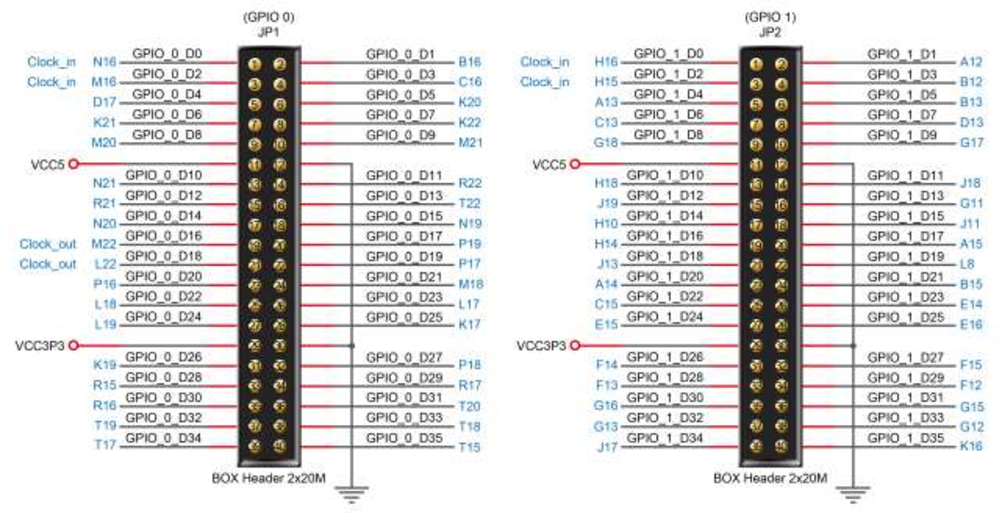
\includegraphics[scale=0.63]{images/de0-cv-gpio}
\caption{Pin assignments of the GPIO headers.}
\label{fig:de0-cv-gpio}
\end{figure}

\subsection{Simulation}
The design can be simulated fully, using QuestaSim Intel Starter or ModelSim Intel Starter. You need a (free) license for QuestaSim. During simulation, all essential signals can be viewed, as is the RAM. The RAM is viewed as 32-bit entries, so we need to do some manual calculations to correctly find byte, half word and word accesses. Simulation can be started from Quartus. Please note that the bootloader must be disabled for normal program start up. 

\subsection{Customizing the design}
\label{sec:customize}
Using VHDL generics, the design can be customized. See Table~\ref{tab:custom}.

\begin{table}[!ht]
\caption{Customization options for the design.}
\label{tab:custom}
\centering
\begin{tabular}{llll}
\toprule
Generic & Type & Default & Comment \\
\midrule
\lstinline|SYSTEM_FREQUENCY| & integer & 50000000 & The system frequency in Hz \\
\lstinline|CLOCK_FREQUENCY| & integer & 1000000 & The clock frequency in Hz \\
\lstinline|HAVE_RISCV_E| & boolean & false & Embedded subset of registers\\
\lstinline|HAVE_MULDIV| & boolean & TRUE &  Hardware multiply/divide \\
\lstinline|FAST_DIVIDE| & boolean & TRUE & Use fast divider\\
\lstinline|HAVE_ZBA| & boolean & false & Use Zba extension \\
\lstinline|VECTORED_MTVEC| & boolean & TRUE & Use vectored interrupts\\
\lstinline|HAVE_REGISTERS_IN_RAM| & boolean & TRUE & Use registers is onboard RAM\\
\lstinline|HAVE_BOOTLOADER_ROM| & boolean & TRUE & Use the bootloader\\
\lstinline|ROM_ADDRESS_BITS| & integer & 16 & ROM size is $2^{16} = 64$ kB \\
\lstinline|RAM_ADDRESS_BITS| & integer & 15 & RAM size is $2^{15} = 32$ kB \\
\lstinline|ROM_HIGH_NIBBLE| & slv(3 downto 0) & x"0" & ROM at 0x0yyyyyyy\\
\lstinline|BOOT_HIGH_NIBBLE| & slv(3 downto 0) & x"1" & Boot at 0x1yyyyyyy\\
\lstinline|RAM_HIGH_NIBBLE| & slv(3 downto 0) & x"2" & RAM at 0x2yyyyyyy\\
\lstinline|IO_HIGH_NIBBLE| & slv(3 downto 0) & x"F" & I/O at 0xFyyyyyyy\\
\lstinline|HAVE_FAST_STORE| & boolean & false & Store takes one clock cycle \\
\lstinline|HAVE_UART1| & boolean & TRUE & Use UART1 \\
\lstinline|HAVE_SPI1| & boolean & TRUE & Use SPI1 \\
\lstinline|HAVE_SPI2| & boolean & TRUE & Use SPI1 \\
\lstinline|HAVE_I2C1| & boolean & TRUE & Use I2C1 \\
\lstinline|HAVE_I2C2| & boolean & TRUE & Use I2C2 \\
\lstinline|HAVE_TIMER1| & boolean & TRUE & Use TIMER1\\
\lstinline|HAVE_TIMER2| & boolean & TRUE & Use TIMER2\\
\bottomrule
\end{tabular}
\end{table}

Notes: leave \lstinline|CLOCK_FREQUENCY| at 1000000. The toolchain depends on it. Also for correct synthesis, \lstinline|SYSTEM_FREQUENCY| must be a integer multiple of \lstinline|CLOCK_FREQUENCY|.
Setting \lstinline|HAVE_FAST_STORE| makes a store \emph{effectively} one clock cycle. The store still needs two clock cycles but the next instruction is executed while the store is taking place. If \lstinline|VECTORED_MTVEC| is set to false, the core cannot execute vectored interrupts.

\section{Cloning the RISC-V project}
\label{sec:cloning}
Now we have to clone the RISC-V project. It incorporates the full Quartus Prime Lite project with the processor written in VHDL. It also incorporates many C program examples and a taylor-made program to convert a RISC-V executable to a VHDL table suitable for the ROM. Create a working directory (and change to that directory) and issue the command:

\begin{lstlisting}[language=]
git clone https:/github.com/jesseopdenbrouw/riscv-rv32
\end{lstlisting}

In the created directory, you will see the following directories:

\lstinline|boards| -- Files needed to use other boards.\\
\lstinline|docs| -- Documentation \\
\lstinline|rtl| -- the VHDL description(s)\\
\lstinline|sw| -- Sample software programs, linker script, library and startup files

Change directory to \lstinline|sw|. Make sure the RISC-V C compiler is available (see Section~\ref{sec:ccompiler}) and is in your path environment variable. Now enter the command \lstinline|make|. It will compile all programs and the support programs \lstinline|srec2vhdl| and \lstinline|upload|. To clean up the programs, issue the command \lstinline|make clean|.

If you want, you can compile the processor with the standard program incorporated, which is by default, flashing onboard leds and writing the current time since last reset via UART1 at 115200 bps. Start your Quartus Prime Lite software and open the project in the \lstinline|rtl| directory. Now start a build by clicking on the play-symbol. It should compile a standard setting (this takes a long time). When finished, you can download the FPGA bitstream file to the DE0-CV board.

To test one of the programs, change directory to one of the directories in \lstinline|sw| and copy the file with \lstinline|.vhd| extension to the directory containing the VHDL description under the name \lstinline|processor_common_rom.vhd|.
Now start Quartus and start the compilation. After a successful compilation, you can program the Cyclone V on a DE0-CV board. If the bootloader is installed, you can also upload an S-record file. See Section~\ref{sec:bootloader}.

The design is targeted for a clock speed of 80\,MHz. Depending on how ``good'' the device is fabricated, higher clock speeds may be obtained. With one device, we could speed up the clock to 133\,MHz.

Compilation of the hardware design is independent of the size of the software program. Several design goals may be selected, such as highest clock speed, minimum power or minimum area. Depending on the compilation settings, compilation time may decrease or increase.


\section{Setting up the GNU C compiler for \textit{this} RISC-V}
\label{sec:ccompiler}
The processor can run C and C++ programs that are compiled using the GNU C/C++ compiler for RISC-V. Besides that, a separate linker script and startup file are needed to setup the compiled code. It is possible to set up the C library for multiple RISC-V architecture versions and select a version during compilation. Building the C/C++ compiler (from Linux) is straightforward:

\begin{enumerate}
\item You need a current GNU C/C++ compiler installed or your Linux box. You also need all essential building tools:
\begin{lstlisting}[language=]
apt install autoconf automake autotools-dev curl python3 libmpc-dev libmpfr-dev libgmp-dev gawk build-essential bison flex texinfo gperf libtool patchutils bc zlib1g-dev libexpat-dev
\end{lstlisting}
\item You need the texinfo package. On Ubuntu et al.\@ issue
\begin{lstlisting}[language=]
apt install texinfo
\end{lstlisting}
\item In your home directory, enter the command
\begin{lstlisting}[language=]
git clone --recursive https://github.com/riscv/riscv-gnu-toolchain
\end{lstlisting}
\item Wait for the cloning to end (takes a long time, about 30 minutes on a Zbook G5 2020 with a 10 MB/s internet connection)
\item Change to the directory with
\begin{lstlisting}[language=]
cd riscv-gnu-toolchain
\end{lstlisting}
\item Make the \lstinline|build| directory with:
\begin{lstlisting}[language=]
mkdir build; cd build
\end{lstlisting}
\item Check the current configuration with
\begin{lstlisting}[language=]
../configure --help | grep abi
\end{lstlisting}
      It should say:
\begin{lstlisting}[language=]
--with-abi=lp64d    Sets the base RISC-V ABI, defaults to lp64d
\end{lstlisting}
The toolchain is currently configured for 64-bit RISC-V. That is not what we want.
\item Enter:
\begin{lstlisting}[language=]
../configure --prefix=/opt/riscv32 --with-arch=rv32im --with-abi=ilp32 --with-multilib-generator="rv32im_zicsr_zba-ilp32--;rv32e-ilp32e--"
\end{lstlisting}
This will set the default architecture to RV32IM, with options for RV32IM with Zicsr and Zba and RV32E (reduced registers, without hardware integer multiply/divide), and the ABI to ilp32 and ilp32e (reduced registers). This means that integers, long integers and pointers use 32-bit entities. The destination directory is \lstinline|/opt/riscv32|.

\item Now enter the \lstinline|make| command: \lstinline|sudo make -j 6|\\
Here \lstinline|make| has to run with supervisor privilege, because the toolchain is put in \lstinline|/opt/riscv32|. This takes a some time (about 15 minutes on a Zbook G5). At some points the compilation seems to hang, but it is just compiling complicated C-files. By the way, you will see a lot of warnings.
\item Now that the toolchain is setup, we have to put the path into the \lstinline|$PATH| environment variable so enter
\begin{lstlisting}[language=]
export PATH=/opt/riscv32/bin:$PATH
\end{lstlisting}
\item Check if the compiler is available:
\begin{lstlisting}[language=]
riscv32-unknown-elf-gcc -v
\end{lstlisting}
It should say something like:
\begin{lstlisting}[language=]
Using built-in specs.
COLLECT_GCC=riscv32-unknown-elf-gcc
COLLECT_LTO_WRAPPER=/opt/riscv32/libexec/gcc/riscv32-unknown-elf/13.2.0/lto-wrapper
Target: riscv32-unknown-elf
Configured with: /home/jesse/riscv-gnu-toolchain/build/../gcc/configure --target=riscv32-unknown-elf --prefix=/opt/riscv32 --disable-shared --disable-threads --enable-languages=c,c++ --with-pkgversion=gc891d8dc23e --with-system-zlib --enable-tls --with-newlib --with-sysroot=/opt/riscv32/riscv32-unknown-elf --with-native-system-header-dir=/include --disable-libmudflap --disable-libssp --disable-libquadmath --disable-libgomp --disable-nls --disable-tm-clone-registry --src=../../gcc --enable-multilib --with-multilib-generator='rv32im_zicsr_zba-ilp32--;rv32e-ilp32e--' --with-abi=ilp32 --with-arch=rv32im --with-tune=rocket --with-isa-spec=20191213 'CFLAGS_FOR_TARGET=-Os    -mcmodel=medlow' 'CXXFLAGS_FOR_TARGET=-Os    -mcmodel=medlow'
Thread model: single
Supported LTO compression algorithms: zlib
gcc version 13.2.0 (gc891d8dc23e) 
\end{lstlisting}
\end{enumerate}

\subsection{Register subset}
It is possible to compile the toolchain to only use register \texttt{x0} to \texttt{x15}. This is called the RISC-V E extension. As a positive side effect, the register file can be cut down from 32 registers to 16 registers, saving 512 memory element. This will lower the ALM count (if placed in ALM flip-flops) and possible speed up the device. A negative side effect is that the pressure on register allocation is higher, possibly increasing instruction count when saving registers on the stack.

Using the above recipe, the toolchain is set up for both RV32IM and RV32E (without hardware integer multiply/divide). You need the specify the architecture and ABI during compile time of the RISC-V programs.

Now compile a C program with:

\begin{lstlisting}[language=]
riscv32-unknown-elf-gcc -O2 -g -o flash flash.c -Wall -T ../ldfiles/riscv.ld -march=rv32e -mabi=ilp32e -nostartfiles --specs=nano.specs ../crt/startup.c
\end{lstlisting}

Make sure to use \lstinline|-march=rv32e| and \lstinline|-mabi=ilp32e|.


\section{Compiling a C program by hand}
We tested a large amount of programs with and without trap handling. We tested all I/O. We did test the use of the C library (\lstinline|malloc| et al, floats and double calculation, some trigonometry functions from the mathematical library), but more tests are needed.

Compiling a program requires the following steps:

\begin{itemize}
\item In the program directory \lstinline|CODE|, create a new directory and change to that directory.
\item Create a C program file, we assume \lstinline|flash.c|.
\item Now issue the command:
\begin{lstlisting}[language=]
riscv32-unknown-elf-gcc -O2 -g -o flash flash.c -Wall -T ../ldfiles/riscv.ld -march=rv32im_zicsr -mabi=ilp32 -nostartfiles --specs=nano.specs ../crt/startup.c
\end{lstlisting}
We supply our own linker file (\lstinline|-T ../ldfiles/riscv.ld|) and we supply our own startup file (\lstinline|../crt/startup.c|). Make sure to use \lstinline|-nostartupfiles| otherwise the default startup file will be linked and errors will report. There a four startup files:
\begin{itemize}
\item \lstinline|empty.S| -- Empty startup file only providing the entry symbol. Can be used with assembler programs. Written in assember.
\item \lstinline|minmal.S| -- Provides the entry symbol, loads the global pointer and stack pointer. Can be used with assembler programs. Written in assembler.
\item \lstinline|simple.S| -- Provides the entry symbol, loads the global pointer and stack pointer and calls \lstinline|main|. On return of \lstinline|main|, it waits in an endless loop. Can be used with minimalistic C programs that do not need global variable initialization and BSS. Written in assembler.
\item \lstinline|startup.c| -- Full support for C programs. Can be used with the standard C library and the mathematical library. Written in C and uses a few assembler instructions.
\end{itemize}
\item Next issue the command:
\begin{lstlisting}[language=]
riscv32-unknown-elf-objcopy -O srec flash flash.srec
\end{lstlisting}
This will create an S-record file in Motorola hex-format.
\item Next issue the command:
\begin{lstlisting}[language=]
../bin/srec2vhdl -wf flash.srec flash.vhd
\end{lstlisting}
This will create a VHDL file with the ROM encoded as 32-bit Little Endian quantities. Note: the taylor-made \lstinline|srec2vhdl| has to be compiled before. See Section~\ref{sec:cloning}.
\item If the bootloader is disabled: issue the command:
\begin{lstlisting}[language=]
cp flash.vhd ../../rtl/thuas-riscv/rom_image.vhd
\end{lstlisting}
This will copy the VHDL file to the RISC-V processor ROM file.
\item Now start the compilation of the VHDL code in Quartus Prime Lite and program the compiled file. This file has the extension \lstinline|.sof|. See Figures~\ref{quartus1} to~\ref{programmer}.
\item If the bootloader is enabled: reset the board to start the bootloader. Then start uploading the S-record file with:
\begin{lstlisting}[language=]
../bin/upload -v flash.srec
\end{lstlisting}
This will upload the file \lstinline|flash.srec| to the board. See also Section~\ref{sec:bootloader}.

\begin{figure}[!ht]
\centering
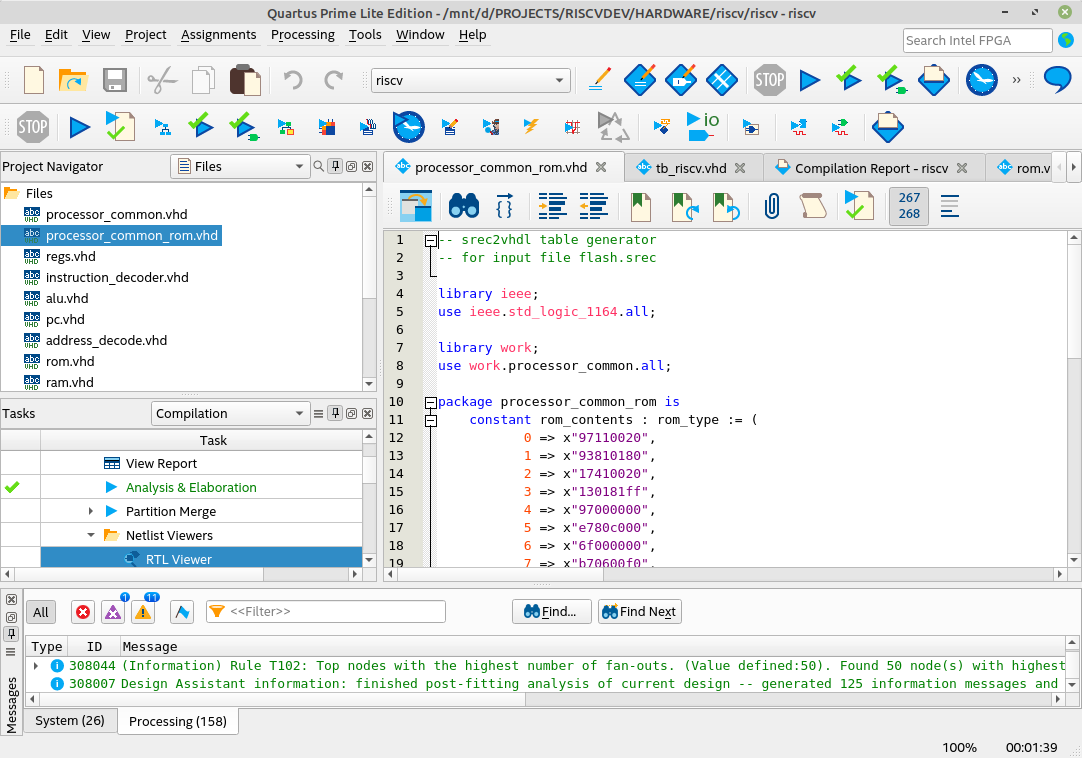
\includegraphics[width=0.85\textwidth]{images/quartus1}
\caption{Image of the Quartus project (1).}
\label{quartus1}
\end{figure}

\begin{figure}[!ht]
\centering
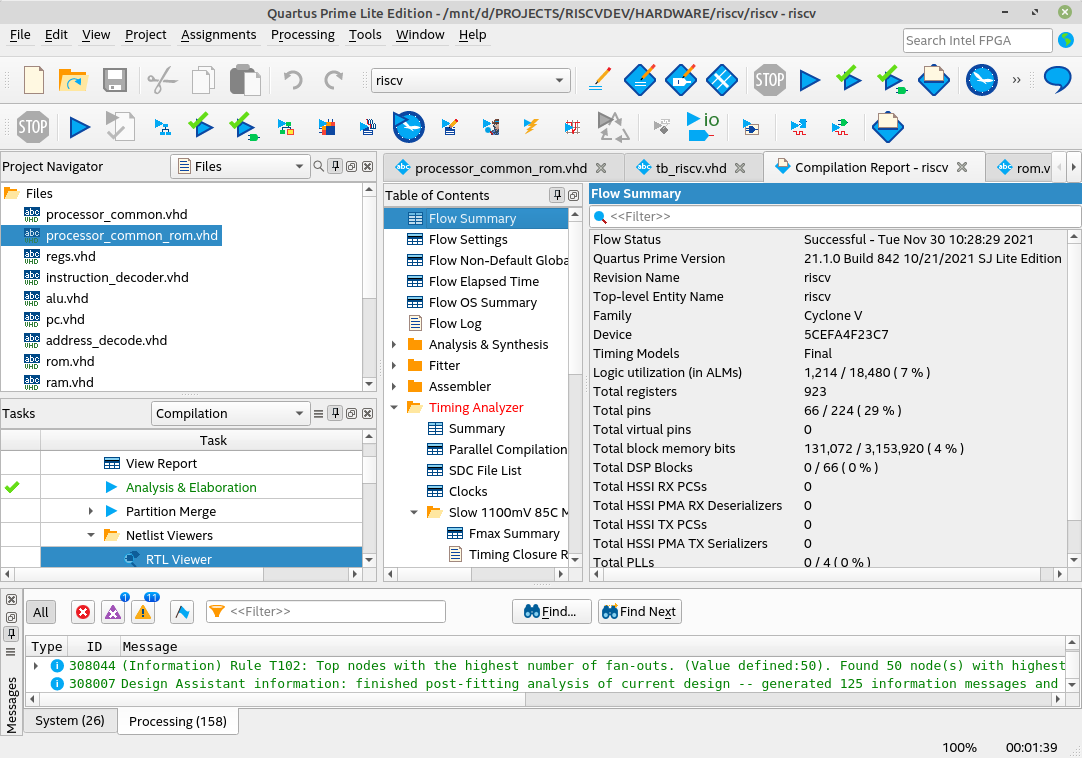
\includegraphics[width=0.85\textwidth]{images/quartus2}
\caption{Image of the Quartus project (2).}
\label{quartus2}
\end{figure}

\begin{figure}[!ht]
\centering
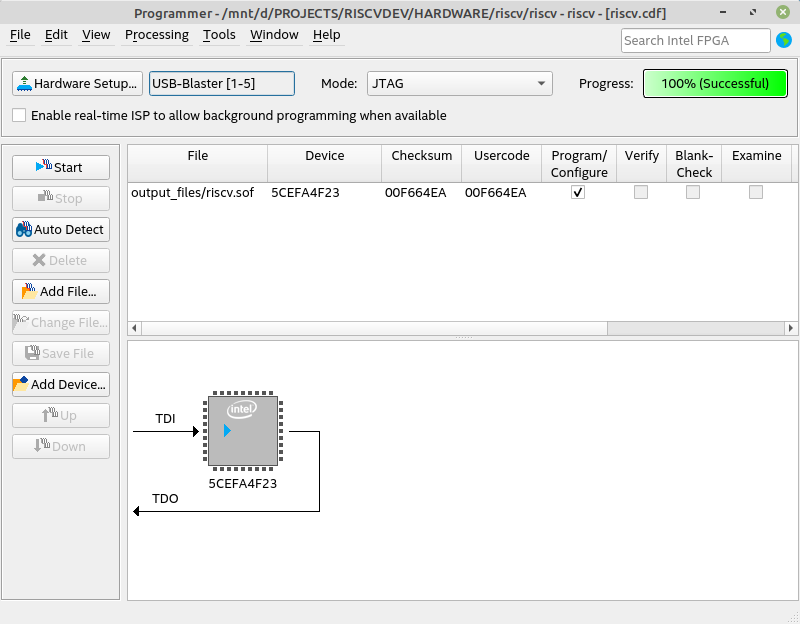
\includegraphics[width=0.85\textwidth]{images/programmer}
\caption{Image of the programmer.}
\label{programmer}
\end{figure}

\end{itemize}

\section{Implemented system calls}
The \lstinline|sbrk| system call, used for allocating RAM memory, is implemented. Note that there is a limited amount of RAM. Note that \lstinline|sbrk| is not called by the user. Use \lstinline|malloc| et al.

The \lstinline|gettimeofday| system call is implemented. It returns the seconds and microseconds since the last reset of the processor. You need to call the \lstinline|gettimeofday| C function for proper handling. %Works with the \lstinline|clock| C library function.

The \lstinline|times| system call is implemented, but only for non-trap system calls. When using trapped systems calls (using ECALL), \lstinline|gettimeofday| is used.

The \lstinline|read| and \lstinline|write| system calls are implemented but in turn they call the userland functions \lstinline|__io_getchar| and \lstinline|__io_putchar| functions to read or write a character. Normal use is for the latter two to transmit or receive via UART1. When implemented, \lstinline|printf| and \lstinline|scanf| can be used.

Other system calls return an error because they cannot fulfill the requested operation, such as \lstinline|open|. Note that some system calls are in fact not implemented and return an error.

Note: when using traps, the system calls are handled by a trap handler (by using ECALL). This is the default behavior of the toolchain. When not using traps, the system calls are rerouted to functions in a library. You need to set up your software properly, in essence provide functions that override the standard C library functions \textit{and} supply two specs files. See the software examples.

\section{Using trap handlers in software}
\label{sec:traphandling}
We provide (see software examples \lstinline|interrupt_direct| and \lstinline|interrupt_vectored|) a basic implementation of trap handlers. In direct mode, the \lstinline|universal_handler| handles all traps (interrupts and exceptions). The entry point (the address loaded in the \lstinline|mtvec| CSR) must be set in the \lstinline|main| function on a 4-byte boundary, as is enabling traps. In vectored mode, interrupts are redirected to their own handlers via a jump table. The start address of the jump table must be set in the \lstinline|main| function on a 4-byte boundary \textit{and} bit 0 of \lstinline|mtvec| must be set to 1, and traps must be enabled. The first entry of the jump table points the universal handler that only handles exceptions. The external timer has its own handler called \lstinline|external_timer_handler|. I2C1 has its own handler called \lstinline|i2c1_handler|. I2C2 has its own handler called \lstinline|i2c2_handler|. TIMER1 has its own handler called \lstinline|timer1_handler|. TIMER2 has its own handler called \lstinline|timer2_handler|. Note that there is only one handler for all four interrupt sources. SPI1 has it own handler called \lstinline|spi1_handler|. UART1 has its own handler called \lstinline|uart1_handler|. This handler is used for both receive and transmit interrupts. Note that negating an interrupt request must be done by software in the respective handlers. The interrupt requests are \emph{not} negated by hardware. Note: the external timer interrupt has to be enabled by writing a 1 to \lstinline|mie.MTIE|. Both software examples implement all available interrupts: SPI1, I2C1, I2C2, TIMER2, UART1, TIMER1 and external system timer. SPI2 doesn't have interrupts. When using traps, you need to set up the trap handler and interrupt service routines.

\paragraph*{Set up traps in direct mode.} The trap handler's entry address must be set up using \lstinline|set_mtvec|. Next, set up the I/O. Then, enable interrupts. The trap handler will be called for both interrupts and exceptions.

\begin{lstlisting}[]
int main(void)
{
    set_mtvec(trap_handler, TRAP_DIRECT_MODE);

    /* do initialization of I/O for interrupts */

    enable_irq();

    /* the rest of the program */
}

__attribute__ ((interrupt))
void trap_handler(void)
{
    /* Trap handler. This is the entry point for both */
    /* interrupts and exceptions. */
}
\end{lstlisting}

\paragraph*{Set up traps is vectored mode.} In vectored mode, interrupts are routed to individual interrupt handlers and exceptions are routed to a common handler. You need a \textsl{jump table} to redirect interrupts to their handlers. The first entry redirects to the handler for execeptions.

\begin{lstlisting}[]
__attribute__ ((naked))
void trap_handler_jump_table(void)
{
    /* Handlers for RISC-V interrupts. Only Machine
     * Timer Interrupt is available. */
    __asm__ volatile ("j trap_handler_vectored;");
    __asm__ volatile ("j default_handler;");
    __asm__ volatile ("j default_handler;");
    __asm__ volatile ("j default_handler;");
    __asm__ volatile ("j default_handler;");
    __asm__ volatile ("j default_handler;");
    __asm__ volatile ("j default_handler;");
    __asm__ volatile ("j external_timer_handler;");
    __asm__ volatile ("j default_handler;");
    __asm__ volatile ("j default_handler;");
    __asm__ volatile ("j default_handler;");
    __asm__ volatile ("j default_handler;");
    __asm__ volatile ("j default_handler;");
    __asm__ volatile ("j default_handler;");
    __asm__ volatile ("j default_handler;");
    __asm__ volatile ("j default_handler;");

    /* Next are the core local interrupts (16 max) */
    __asm__ volatile ("j default_handler;");
    __asm__ volatile ("j default_handler;");
    __asm__ volatile ("j external_input_handler;");
    __asm__ volatile ("j default_handler;");
    __asm__ volatile ("j timer1_handler;");
    __asm__ volatile ("j timer2_handler;");
    __asm__ volatile ("j default_handler;");
    __asm__ volatile ("j uart1_handler;");
    __asm__ volatile ("j i2c2_handler;");
    __asm__ volatile ("j default_handler;");
    __asm__ volatile ("j i2c1_handler;");
    __asm__ volatile ("j spi1_handler;");
    __asm__ volatile ("j default_handler;");
    __asm__ volatile ("j default_handler;");
    __asm__ volatile ("j default_handler;");
    __asm__ volatile ("j default_handler;");
}

int main(void)
{
    set_mtvec(handler_jump_table, TRAP_VECTORED_MODE);

    /* do initialization of I/O for interrupts */

    enable_irq();

    /* the rest of the program */
}

__attribute__ ((interrupt))
void exception_handler(void)
{
    /* Excpetion handler. This is the entry point for */
    /* exceptions, not for interrupts */
}

__attribute__ ((interrupt))
void default_handler(void)
{
    while (1);
}

__attribute__ ((interrupt))
void timer1_handler(void)
{
    /* Do something */
}

/* ... other handlers here ... */
\end{lstlisting}

%set_mtvec(jumptable, TRAP_VECTORED_MODE);

\section{Software programs}
The \lstinline|sw| directory contains programs that run on this RISC-V processor. Under Linux, change to the \lstinline|sw| directory and issue the \lstinline|make| command. Now all programs are compiled as is a THUAS-specific library. To upload a program to the RISC-V processor, change to one of the program directories and issue the command \lstinline|make upload|. This will upload the corresponding S-record file to the processor using UART1. Make sure no terminal program (e.g.\@ PuTTY) is connected. The bootloader hardware must be installed. See Section~\ref{sec:bootloader}.

After \lstinline|make| is run, a static library called \lstinline|libthuasrv32.a| is available with functions to use the I/O and trap related functions. You need to supply the library to the linker. Also, two \lstinline|specs| files are available. Use \lstinline|--specs=<path-to>/thuas.specs| for including the THUAS library and use \lstinline|--specs=<path-to>/nano.specs| for including the \lstinline|nano| library \textsl{without} the \lstinline|gloss| library (used for \lstinline|ECALL|-driven system calls). If you need \lstinline|ECAll|-driven system calls, use \lstinline|--specs=nano.specs| (without a path name) to use the RISC-V specific \lstinline|nano| library \textsl{with} the \lstinline|gloss| library.

In the \lstinline|sw| directory, there are a number of software programs available. First, the common files:

\begin{itemize}
\item \lstinline|ldfiles| -- contains the linker scripts. There are three scripts:
\begin{itemize}
\item \lstinline|riscv.ld| -- default linker script: ROM = 64 kB, RAM = 32 kB, I/O = 16 kB.
\item \lstinline|riscv-largerom.ld| -- linker script with enlarged ROM: ROM = 128 kB, RAM = 32 kB, I/O = 16 kB. You need to update the ROM settings in the hardware.
\item \lstinline|riscv-big.ld| -- linker script with enlarged ROM and RAM: ROM = 128 kB, RAM = 64 kB, I/O = 16 kB. You need to update the ROM and RAM settings in the hardware.
\end{itemize}
\item \lstinline|crt| -- contains the startup files.
\item \lstinline|bin| -- contains the binaries of \lstinline|srec2vhdl| and \lstinline|upload|. This directory is created when running \lstinline|make|.
\item \lstinline|include| -- contains the header files for the design. Use \lstinline|#include <thuasrv32.h>| in programs.
\item \lstinline|lib| -- contains the libraries for the design. Link against \lstinline|libthuasrv32.a|.
\end{itemize}

Some examples are to be used in de simulator only, mainly to test functionality and clock cycle accuracy. Most examples work on the DE0-CV board, but without testing traps. Two examples work on the board and use traps.

\begin{itemize}
\item \lstinline|add64| -- simple 64-bit addition. For use in the simulator.
\item \lstinline|assembler| -- a simple assembler program. For use in the simulator.
\item \lstinline|basel_problem| -- a program that calculates the sum of the inverses of the squares of natural numbers, up to 1000. For use in the simulator. Used to test the divider.
\item \lstinline|bootloader| -- the bootloader program, placed in the bootloader ROM. It has separate startup and linker files. Uses UART1. Works on the board.
\item \lstinline|clock| -- a simple clock using the CSR MTIME and MTIMEH registers to fetch the time since last reset. Uses UART1. Works on the board.
\item \lstinline|coremark| -- implementation of the CoreMark test suite. Uses UART1. Works on the board.
\item \lstinline|ctor_c| -- C test to check if global constructors are called upon program execution. Uses UART1. Works on the board.
\item \lstinline|ctor_cpp| -- C++ test to check if global constructors are called upon program execution. Uses UART1. Works on the board.
\item \lstinline|dhrystone| -- preliminary Dhrystone test suite. Works on the board.
\item \lstinline|double| -- some floating point double computations. For simulation.
\item \lstinline|exp| -- calculates Euler's number e. For simulation.
\item \lstinline|fatfs| -- implementation of FATFS\footnote{\url{http://elm-chan.org/fsw/ff/00index_e.html}}, supports read/write, long filename, codepage 437 (US). FAT16, FAT32 supported. exFAT not tested. Works on the board.
\item \lstinline|flash| -- flash the DE0-CV board leds, works on the board.
\item \lstinline|float| -- some floating point float computations. For simulation.
\item \lstinline|FreeRTOSdemo| -- implementation of blinky demo and full demo of the FreeRTOS real-time operating system. Works on the board. Needs more tests with interrupts.
\item \lstinline|global| -- test for globals and local statics with initialization. For simulation
\item \lstinline|hex_display| -- program that reads 8 switches from the board and display them as a 2-digit hexadecimal value on the 7-segment display. Works on the board. Note that on the DE0-CV board, the decimal points cannot be used, because they are not connected to FPGA pins.
\item \lstinline|i2c1findslaves| -- program that uses the I2C1 peripheral to find slaves on the I\textsuperscript{2}C bus. Prints out the found slaves addresses on the terminal. Works on the board.
\item \lstinline|i2c1lis3dh| -- program to read acceleration data from a LIS3DH accelerometer. Uses I2C1 and UART1. Works on the board.
\item \lstinline|i2c1ssd1315| -- program to test the SSD1315 OLED display driver. Uses I2C1 and UART1. Works on the board.
\item \lstinline|i2c1tmp102| -- program that uses the I2C1 peripheral to fetch the temperature data of a TMP102 temperature sensor and displays the raw data on the terminal. Works on the board.
\item \lstinline|interrupt_direct| -- program to test the interrupt handling using direct mode and prints out the elapsed time. Uses UART1. Works on the board.
\item \lstinline|interrupt_vectored| -- program to test the interrupt handling using vectored mode.and prints out the elapsed time. Uses UART1. Works on the board.
\item \lstinline|interval| -- program that uses the \lstinline|clock| C library function to time 5 seconds since last read. Uses UART1. Works on the board.
\item \lstinline|ioadd| -- adds the lower 5 switches to the upper 5 switches and displays the result on the leds. Tests addition, shifting and I/O. Works on the board.
\item \lstinline|linked_list| -- example on how to use linked lists. This program soups up all available dynamic RAM but does not penetrate the reserved stack space. Uses UART1. Works on the board.
\item \lstinline|malloc| -- example to test \lstinline|malloc| and friends. Works. Used in simulations.
\item \lstinline|mcountinhibit| -- program to test the \lstinline|mcountinhibit| CSR. Uses UART1. Works on the board.
\item \lstinline|monitor| -- simple monitor program. Works on the board. Uses strings, UART1, RAM, ROM, I/O and \lstinline|sprintf| (and therefore \lstinline|malloc| et al.).
\item \lstinline|mult| -- integer multiplication with the C library. Set to the E extension with no hardware multiply/divide support. For simulations.
\item \lstinline|mxhw| -- Program to read out the \lstinline|mxhw| and \lstinline|mxspeed| custom CSRs and print the hardware configuration and clock speed of the synthesized processor to the terminal.
\item \lstinline|qsort| -- sorts an integer array using the \lstinline|qsort| C library function and prints the result to UART1. Works on the DE0-CV board.
\item \lstinline|riemann_left| -- calculates the Riemann Left Sum of $\sin^2 x$ from $0$ to $2\pi$. For use in the simulator. The  result must be $\pi$.
\item \lstinline|shift| -- shifts. For use in simulations.
\item \lstinline|spi1readeeprom| -- using the SPI1 peripheral to read out 16 bytes of the 25AA010A EEPROM slave, one byte at the time, using hardware Slave Select. Uses UART1. Works on the board.
\item \lstinline|spi1softnss| -- as \lstinline|spi1readeeprom|, using software Slave Select.
\item \lstinline|spi1speed| -- using the SPI1 peripheral to read out (full speed) 16 bytes of the 25AA010A EEPROM slave, using hardware Slave Select. Uses UART1. Works on the board.
\item \lstinline|spi1writeeeprom| -- using the SPI1 peripheral to write and read out (full speed) the 25AA010A EEPROM slave, using software Slave Select. Uses UART1. Works on the board.
\item \lstinline|sprintf| -- prints integers, floats/doubles to a string. This is a big binary. For simulations.
\item \lstinline|string| -- some string functions. For simulations.
\item \lstinline|testexceptions| -- program that tests all implemented exceptions. Works on the board.
\item \lstinline|testio| -- simple program that copies the input (switches) to the output (leds). Works on the board.
\item \lstinline|timer1| -- a simple program that uses TIMER1 interrupt to generate a time base for an interrupt handler. Shows how to set up direct mode interrupts. Works on the board.
\item \lstinline|timer2pwm| -- Shows how use TIMER2's PWM and Output Compare feature. Works on the board.
\item \lstinline|timer2ic| -- Shows how use TIMER2's Input Capture feature. Works on the board.
\item \lstinline|trig| -- some float trigonometry functions for float and double. Prints results to UART1. This is a big binary.
\item \lstinline|upload| -- a Linux/PC program to upload an S-record file using the bootloader.
\item \lstinline|uart_cpp| -- Simple C++ UART program. Makes use of a singleton design pattern. Works on the board.
\item \lstinline|uart_printf| -- simple program that prints an integer, a pointer, a float and a double to the terminal using \lstinline|printf|, this is a big binary. Works on the board.
\item \lstinline|uart1_printlonglong| -- program that prints a long long and unsigned long long to the UART. Works on the board.
\item \lstinline|uart_sprintf| -- simple program that prints an integer, a pointer, a float and a double to the terminal, this is a big binary. Works on the board.
\item \lstinline|uart_test| -- simple UART1 program. Works on the board.
\end{itemize} 

Note: we use a lot of the \lstinline|volatile| keyword to emit the variables to RAM for easy inspection in the simulator. You will see compiler warnings from C library functions.

Note that the floating point programs loads (huge) functions from the C library and possibly create a binary that is too large to fit in the ROM. In that case, the linker will issue an error and does not build the binary. You have to update the data sizes in the VHDL description and select a suitable linker script.

When using floats and doubles in \lstinline|sprintf|/\lstinline|printf|, you need to supply the linker with the \lstinline|-u _printf_float| option. When using floats and doubles in \lstinline|sscanf|/\lstinline|scanf|, you need to supply the linker with the \lstinline|-u _scanf_float| option. Also, using \lstinline|printf| and \lstinline|scanf| create big binaries.

Note that \lstinline|sprintf|/\lstinline|printf| do not print 64-bit integers (a.k.a.\@ \lstinline|long long|) because of lack of support in the \lstinline|nano| library.

\subsection{srec2vhdl}
This is a homebrew utility to convert a Motorola S-record file into a VHDL file suitable for inclusion of the processor. The program is called with:

\begin{lstlisting}[language=]
srec2vhdl [-fbwhqvd0] [-i <arg>] inputfile [outputfile]
\end{lstlisting}

\lstinline|inputfile| is the S-record file, created by the \lstinline|objdump| program. \lstinline|outputfile| is the VHDL output file. When omitted, \lstinline|stdout| is used. There are a number of options:

\begin{itemize}
\item \lstinline|-f| makes a full output that directly can be used. If not used, only the ROM table contents itself is produced.
\item \lstinline|-w| ROM contents is in words (32 bits).
\item \lstinline|-h| ROM contents is in half words (16 bits).
\item \lstinline|-b| ROM contents is in bytes (8 bits).
\item \lstinline|-v| Verbose output.
\item \lstinline|-d| Output unused ROM data as don't care.
\item \lstinline|-0| Output unused ROM data as 0.
\item \lstinline|-q| Quiet output, only error messages are displayed.
\item \lstinline|-i <arg>| indents each line with \lstinline|<arg>| spaces.
\end{itemize}

Note: unused ROM addresses are not output, except when the \lstinline|-0| or \lstinline|-d| options are used.
%\subsection{Monitor program}
%A simple monitor program is available, see the \lstinline|monitor| directory in software examples. It makes use of UART1. You need a terminal program like Putty and a U(S)ART to USB device for your computer. Currently the following commands are available:
%
%\begin{itemize}
%\item \lstinline|l| -- set Little Endian (default),
%\item \lstinline|b| -- set Big endian.
%\item \lstinline|rw <address>| -- read word at address (4-byte boundary),
%\item \lstinline|rh <address>| -- read half word at address (2-byte boundary),
%\item \lstinline|rb <address>| -- read byte at address,
%\item \lstinline|ww <address> <data>| -- write word at address (4-byte boundary),
%\item \lstinline|wh <address> <data>| -- write half word at address (2-byte boundary),
%\item \lstinline|wb <address> <data>| -- write byte at address,
%\end{itemize}
%
%\lstinline|<address>| and \lstinline|<data>| in hexadecimal and Big Endian format. For ROM and RAM read accesses, best set to Little Endian. For I/O accesses, set Big Endian. Make sure to read and write I/O as words. Note that ROM cannot be written.

\section{Address ranges and memory sizes}
The processor uses a 32-bit linear address space (4 GB) and is divided in 16 blocks of 256 MB each. The top four bits (31 to 28) select a block while the remaining bits select the address within a block.
By default, the ROM starts at address 0x00000000 and and has a size of 64 kB (16 k words). The Program Counter then starts at 0x00000000. The bootloader ROM starts at address 0x10000000 and has a size of 4 kB (1 k words). The Program Counter then starts at address 0x10000000. The RAM starts at address 0x20000000 and has a size of 32 kB (8 k words). The stack pointer is set to one address above the last RAM byte, by default at 0x20008000. The I/O starts at address 0xF0000000 and has a size of 16 kB (4 k words).

The ROM, bootloader ROM, RAM and I/O may be moved to another start location. The Program Counter is started at the correct address. The placement of the ROM is in 256 MB intervals, which are the 4 most significant bits of a 32-bit address. The same holds for the RAM and the I/O. To move the memories, find the toplevel of the \lstinline|riscv|-entity. There you will see the following generics:

\lstinputlisting[language=C,breaklines=false,linerange={25-32}]{code/riscv.vhd}

Change the start locations of the memories by changing the constants. Make sure the memories do not overlap. To change the sizes of the ROM and the RAM, look for the lines as shown below:

\lstinputlisting[language=C,breaklines=false,linerange={21-24}]{code/riscv.vhd}

Note that you also have to make changes to the linker script. In the file \lstinline|riscv.ld|, at the top you will find the following lines. Change the origins in accordance with the VHDL description.

\begin{lstlisting}
ENTRY( _start )

MEMORY
{
   ROM (rx)   : ORIGIN = 0x00000000, LENGTH = 64K
   RAM (rw)   : ORIGIN = 0x20000000, LENGTH = 32K
   IO (rw)    : ORIGIN = 0xf0000000, LENGTH = 16K
}
\end{lstlisting}

In this setting, the ROM is 64 kB long and the RAM is 32 kB long. Please note that both ROM and RAM bits may not exceed 3,153,920 bits of onboard RAM. For increased ROM and RAM size, typical values may be 128 kB ROM and 64 kB RAM.

Note that we do not use full address decoding for ROM, boot ROM, RAM and I/O. This means that, for example, the ROM is visible multiple times in the address space. This is called \emph{memory foldback}. For the ROM this is at 64 kB intervals. So the contents of address 0x00000000 is also available at address 0x00010000.

\section{Using the bootloader}
\label{sec:bootloader}
The design incorporates a hard-coded bootloader with an upload and a simple monitor program. The bootloader is placed in a separate ROM starting at address 0x10000000 and has a maximum length of 4 KB (may be extended). The bootloader cannot be overwritten by an upload. The bootloader can be disabled.

\subsection{S-record file}
The S-record standard is invented by Motorola in the 1980's. It consists of formatted lines, called records. Each line can be seen as a record. A record starts with \lstinline|S| followed by a single digit. \lstinline|S0| is used as header record. This record is ignored by the bootloader. \lstinline|S1|,  \lstinline|S2| and \lstinline|S3| are data record using a 2-byte, 3-byte and 4-byte start address respectively. \lstinline|S4| is reserved and skipped by the bootloader. \lstinline|S5| and \lstinline|S6| are count records and are ignored. \lstinline|S7|, \lstinline|S8| and \lstinline|S9| are termination records with a start address incorporated, with 4-byte, 3-byte and 2-byte address respectively. This start address is used by the bootloader to start the application. Records have a checksum at the end, this checksum is ignored by the bootloader.

\subsection{Startup sequence}
After loading the design in the FPGA, or after resetting the FPGA, the bootloader starts. It presents itself with a welcome string printed via UART1 at default 115200 bps. Then the bootloader waits for about 5 seconds before starting the application at address 0x00000000. During these 5 seconds, at half second intervals, a \lstinline|*| is printed via UART1. At the same time, the 10 red leds on the DE0-CV board are lit and dimmed on half second intervals from left (high led) to right (low led). If a character is received within the five seconds, either a S-record file can be uploaded or the bootloader falls to a simple monitor program.

\subsection{Uploading an S-record file}
A Motorola S-record file can be uploaded with the \lstinline|upload| program found in the \lstinline|sw| directory. It is tested on Linux, Windows is currently not supported. S-record files for all RISC-V programs are generated as part of the \lstinline|make| process by the RISC-V \lstinline|objcopy| program. The \lstinline|upload| program is invoked with:

\begin{lstlisting}[language=]
upload -d <device> -b <baud> -t <timeout> -s <sleep> -vjn file
\end{lstlisting}

The default device is \lstinline|/dev/ttyUSB0| which is the first plugged-in USB-to-U(S)ART converter. The baudrate may be 9600 bps or 115200 bps (default). Timeout is the time the \lstinline|uplead| program waits for expected data from the bootloader. The time is set in deciseconds (0.1 seconds) intervals. The default value is 10 (1.0 seconds). Sleep is the time the \lstinline|upload| program waits after transmitting a character to the bootloader in microseconds intervals. The default value is 0. The option \lstinline|-v| turns on verbose mode. The option \lstinline[]|-j| instructs \lstinline|upload| to send a ``start application'' command to the bootloader after the S-record file is uploaded. The option \lstinline|-n| disables handshake with the bootloader. File must be a valid S-record file.

To upload an S-record file, reset the FPGA or program the FPGA design in the FPGA. Then, within the 5 seconds interval, start the \lstinline|upload| program with options and file name supplied. If the \lstinline|upload| programs manages the contact the bootloader, the S-record file will be uploaded. Depending on the size, uploading may take as short as a few seconds to minutes for a large file. As a rule of thumb, about 2400 file characters per seconds are send (at 115200 bps). Make sure that \emph{no} terminal program (e.g.\@ PuTTY) is active. If the \lstinline|upload| program cannot contact the bootloader, it exits with an error message. If during sending the records, a response from the bootloader is not read, the \lstinline|upload| exits with an error message. This is mostly due to an open terminal connection. To start the application after the upload, supply the \lstinline|-j| option to the \lstinline|upload| program, otherwise the monitor is started. Before starting the application, UART1 is turned off and the output port is set to 0x00000000 (i.e.\@ all port bits are set to 0).

Using an USB-to-serial adapter can be troublesome, for example when stopping (Ctrl-C) the upload program. There will be characters in the USB buffer and the upload program and the bootloader will be out of sync. Best is to remove the USB-to-serial adapter from the PC and reinsert it again. Then the USB buffer will be empty. During the transmission, the low led of the DE0-CV board will flash rapidly. If not, there is no upload and the USB-to-serial adapter and the DE0-CV board are out of sync.

\subsection{Using the monitor}
If within the 5 seconds grace period a character is received by the bootloader, the bootloader falls to a simple monitor program. The monitor recognized some simple commands. Each command is terminated by an enter key.

\lstinline|r|

Run the program at address 0x00000000.

\lstinline|rw <address>|

Read and print word at address. Address must be on a 4-byte boundary. Data is presented in big endian.

\lstinline|dw <address>|

Dump 16 words from memory to the terminal. Address must be on a 4-byte boundary. After each word, 4 ASCII characters are printed, if printable. If not printable, a dot is printed. Useful for finding strings in memory. Data is presented in big endian.

\lstinline|n|

Dump next 16 words from memory to the terminal, and ASCII characters.

\lstinline|ww <address> <data>|

Write 4-byte data at address. Address must be on a 4-byte boundary. Data must be in big endian.

\lstinline|h|

A simple help menu is presented.

Note: the capabilities of the monitor may be extended.

\subsection{Upload protocol}
(When not using the \lstinline|-n| option) Uploading an S-record file uses a simple handshake protocol. The \lstinline|upload| program sends a single exclamation mark (\lstinline|!|). The bootloader responds with an question mark (\lstinline|?|) and a newline (\lstinline|\n|). Now each S-record line is transmitted character by character, including the end-of-line termination character (\lstinline|\r| and/or \lstinline|\n|). After a line is processed, the bootloader responds with a question mark and a newline. After all S-record lines are transmitted, the \lstinline|upload| program either sends a \lstinline|J| to start the application, or a \lstinline|#| to start the monitor.

(When using the \lstinline|-n| option) The \lstinline|upload| program transmits n dollar sign (\lstinline|$|) to inform the bootloader that handshake is turned off. The \lstinline|upload| program then transmits the S-record file and doesn't wait for acknowledge (the bootloader will not send an acknowledge). This provides a fast upload scenario (about 4 times faster then when using acknowledge).

\subsection{Implications on the hardware design}
The design has a separate ROM that incorporates the bootloader. The original ROM, at address 0x00000000 is extended with a write port, together with the instruction read port and the data read port. In fact, the ROM has become a (program) RAM. Because the Cyclone FPGA ROMs (and RAMs) can only have two ports (out/out or in/out), the original ROM hardware is duplicated (by the synthesizer). This takes up onboard RAM blocks, but very few ALMs (cells). % The speed decrements by a few MHz.

Note that the ROM can only be (over)written with words on a 4-byte boundary.

\section{Future plans (or not) and issues}
Some future plans:

\begin{itemize}
\item We are \emph{not} planning the C standard.
\item The CSR is almost conform the standard.
\item Implement clock stretching and arbitration in the I\textsuperscript{2}C peripherals.
\item Adding input synchronization for SPI1 and SPI2 peripherals.
\item Implement an I/O input/output multiplexer for \lstinline|gpioapin| and \lstinline|gpioapout|. This will enable I/O functions to be multiplexed with normal port I/O.
\item Implement I/O with selectable for input or output. This implies tri-state buffers and some synthesizer don't want these buried in a hierarchy.
\item Smaller (in cells) divide unit.
\item Adding the Zbb extension.
\item Test more functions of the standard and mathematical libraries.
\item It is not possible to print \lstinline|long long| (i.e. 64-bit) using \lstinline|printf| et al. When using the format specifier \lstinline|%lld|, \lstinline|printf| just prints \lstinline|ld|. This due to lack of support in the \lstinline|nano| library.

\end{itemize}

\appendix
\section{C Runtime startup code}
Before \lstinline|main| is called, the C Runtime startup code (normally in a file called \lstinline|crt0.s|, maybe we change that in the future) does some initialization:

\begin{itemize}
\item Set up the trap vector address to catch early traps.
\item Load the Stack Pointer with the end address +1 of the RAM.
\item Load the Global Pointer with a suitable address.
\item Initialize (clear) the BBS section with 0, for globals/statics without initialization.
\item Initialize globals/statics \emph{with} initialization.
\item Call the global constructors.
\item Call \lstinline|main|.
\item Call the global destructors.
\item Call \lstinline|exit|.
\end{itemize} 

Although this is a bare metal processor, without an operating system, it is possible to pass arguments (\lstinline|argc|, \lstinline|argv|) to \lstinline|main|. This is shown in de code below. When the linker links all object files to an executable, it sets the entry point to a symbol called \lstinline|_start|. So our C Runtime startup is a function called \lstinline|_start|. It has no parameters and doesn't return anything. Furthermore, the function must not use the stack and be placed at the begin of the ROM. The linker file (\lstinline|riscv.ld|) supplies the linker with some symbols: \lstinline|_sbbs| and \lstinline|_ebbs| have the addresses of the BBS section (in RAM). The initialization data of the initialized globals/statics are within the ROM code and must be copied to the RAM before \lstinline|main| starts. The data starts at the address found in symbol \lstinline|_sidata| and must be copies to RAM memory available in symbols \lstinline|_sdata| and \lstinline|_edata|.
When using register variables, the C compiler will detect loops for BSS zeroing and copying ROM data to RAM and will use \lstinline|memset| and \lstinline|memcpy| to perform the actions.

\lstinputlisting[aboveskip=2ex,language=C,breaklines=false]{code/startup.c}

\section{The I/O at a glance}

The I/O registers are directly addressable or by a struct. See the listing below.

\lstinputlisting[language=C,breaklines=false]{code/io.h}

\section{Port I/O}
The processor is equipped with a single 32-bit input and 32-bit output port. There is no data direction register. This may be changed to using bi-direction port pins. Note that all accesses on the I/O are in Big Endian. This means that bit 31 of the input will be placed in bit 31 of the used variable.

To set the outputs, use:

\begin{lstlisting}[language=C]
uint32_t output = 0xff00ff00;

GPIOA->POUT = output;
\end{lstlisting}

Modifying bits of a I/O register must be done by a read-modify-write cycle. This is \emph{not} atomically handled and can interfere with interrupts! For example, to set bit 2 of POUT, use:

\begin{lstlisting}[language=C]
GPIOA->POUT |= 0x04;
\end{lstlisting}

\section{UART1 Code}

UART1 can send and receive data with one start bit, 7/8/9 data bits, N/E/O parity and 1 or 2 stop bits. Transmission is tested with a baud rate of 9600 bps, 115200 bps and 230400 bps. Send and receive speeds are equal as is the number of data bits, parity and the number of stop bits. There are no auxiliary control signals (e.g. RTS and CTS). There is no embedded FIFO to buffer incoming data. UART1 is programmable using I/O registers, see Appendix~\ref{sec:ioregisters}. Note that using a system frequency of 50 MHz, the baud rate cannot be lower than 763 bps, because the baud rate generator uses a 16-bit register.

To initialize UART1, use the code in the listing below:

\begin{lstlisting}[language=C]
/* Frequency of the DE0-CV board */
#define F_CPU (50000000UL)
/* Transmission speed */
#define BAUD_RATE (9600UL)

/* Initialize the Baud Rate Generator */
void UART1_init(void)
{
    /* Set baud rate generator */
    UART1->BAUD = F_CPU/BAUD_RATE-1;
}
\end{lstlisting}

To send a single character with waiting, use the code in the listing below:

\begin{lstlisting}[language=C]
/* Send one character over UART1 */
void uart1_putc(int ch)
{
    /* Transmit data */
    UART1->DATA = (uint8_t) ch;
            
    /* Wait for transmission end */
    while ((UART1->STAT & 0x10) == 0);
}
\end{lstlisting}

To send a null-terminated string, use the code in the listing below:

\begin{lstlisting}[language=C]
/* Send a null-terminated string over UART1 */
void uart1_puts(char *s)
{
    if (s == NULL)
    {
        return;
    }

    while (*s != '\0')
    {
        uart1_putc(*s++);
    }
}
\end{lstlisting}

To wait for a character reception, use the code in the listing below:

\begin{lstlisting}[language=C]
/* Get one character from UART1 in
 * blocking mode */
int uart1_getc(void)
{
    /* Wait for received character */
    while ((UART1->STAT & 0x04) == 0);

    /* Return 8-bit data */
    return UART1->DATA & 0x000000ff;
}
\end{lstlisting}

To receive a string from UART1, including some simple line editing, use the code in the listing below:

\begin{lstlisting}[language=C]
/* Gets a string terminated by a newline character from UART1
 * The newline character is not part of the returned string.
 * The string is null-terminated.
 * A maximum of size-1 characters are read.
 * Some simple line handling is implemented */
int uart1_gets(char buffer[], int size)
{
	int index = 0;
	char chr;

	while (1) {
		chr = uart1_getc();
		switch (chr) {
			case '\n':
			case '\r': buffer[index] = '\0';
					   uart1_puts("\r\n");
					   return index;
					   break;
			/* Backspace key */
			case 0x7f:
			case '\b': if (index>0) {
						   uart1_putc(0x7f);
						   index--;
					   } else {
					       uart1_putc('\a');
				       }
					   break;
			/* control-U */
			case 21:   while (index>0) {
					       uart1_putc(0x7f);
						   index--;
					   }
					   break;
			/* control-C */
			case 0x03: uart1_puts("<break>\r\n");
					   index=0;
					   break;
			default:   if (index<size-1) {
					       if (chr>0x1f && chr<0x7f) {
						       buffer[index] = chr;
							   index++;
							   uart1_putc(chr);
						   }
					   } else {
						   uart1_putc('\a');
					   }
					   break;
		}
	}
	return index;
}
\end{lstlisting}

When printing a C newline, you have to use:

\begin{lstlisting}[language=C]
uart1_puts("\r\n");
\end{lstlisting}

This will set the cursor to the beginning of a new line. Here, \lstinline|\r| returns the cursor to the beginning of the current line and \lstinline|\n| advances the cursor to the next line. Some terminal emulation programs can be instructed to move to the beginning of a new line with only \lstinline|\n|.

For working with the UART on board of the processor, you need an USB-to-U(S)ART device with TTL (3.3 V) converter. An example is shown in Figure~\ref{fig:usb-usart-ttl}.

\begin{figure}[!ht]
\centering
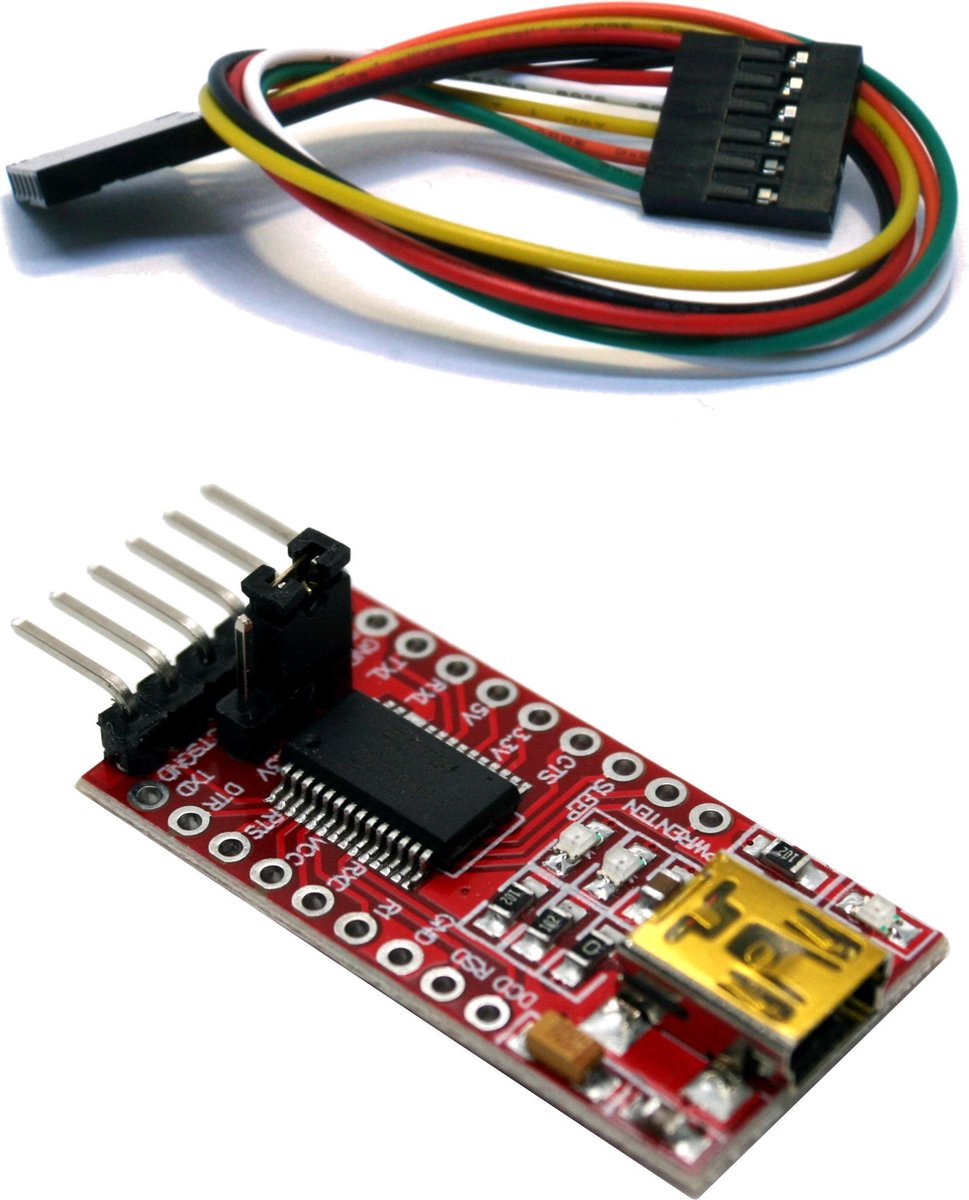
\includegraphics[scale=0.1]{images/usb-usart-ttl}
\caption{An USB-to-U(S)ART converter. Make sure that the voltages do not exceed 3.3 V.}
\label{fig:usb-usart-ttl}
\end{figure}


\section{I\textsuperscript{2}C code}
The baud rate prescaler must be loaded with the number of system clock cycles for \textbf{one-half} bit time minus 1 for Standard mode, and \textbf{one-third} bit time minus 1 for Fast mode. Note that the prescaler is in the CTRL register and must be preserved:

\begin{lstlisting}[caption=]
/* Standard mode, exact number */
#define TRAN_SPEED ((F_CPU/2UL/100000UL)-1)
I2C1->CTRL = TRAN_SPEED << 16;
/* Fast mode, round up to integer */
#define TRAN_SPEED ((F_CPU/3UL/400000UL)-1)
I2C1->CTRL = (TRAN_SPEED << 16) | (1 << 2);
\end{lstlisting} 

Note that for a 50\,MHz system clock frequency, an exact count is achieved for Standard Mode (250), but not for Fast mode (41.6667), so the rounding must be up.

To send a START, before an address byte is send, use:

\begin{lstlisting}[caption=]
I2C1->CTRL |= (1 << 9);
\end{lstlisting} 

Then, to send an address byte, with read-write bit, \textbf{left-shift the address by 1} and add the read/write bit:

\begin{lstlisting}[caption=]
I2C1->DATA = (ADDR << 1) | RWBIT;
while ((I2C1->STAT & 0x08) == 0x00);
\end{lstlisting} 

To check for acknowledge, use:

\begin{lstlisting}[caption=]
if (I2C1->STAT & (1 << 5)) {
    uart1_puts("ACK failed!\r\n");
} else {
    uart1_puts("ACK ok\r\n");
}
\end{lstlisting} 

To send a byte and wait for transmission complete, use:

\begin{lstlisting}[caption=]
I2C1->DATA = some_data;
while ((I2C1->STAT & 0x08) == 0x00);
\end{lstlisting} 

To receive a byte, the controller must issue a series of clock pulses, but mustn't write any data. This is done by transmitting a dummy byte with the contents 0xff. Because of the open-drain bus lines, this will let the target to determine the logic values. Except for the last byte received, all transmissions must be acknowledged by the controller. Therefore, the MACK (master acknowledge) bit must be set.

\begin{lstlisting}[caption=]
/* Set MACK bit */
I2C1->CTRL |= (1 << 11);
/* Controller is receiving */
I2C1->DATA = 0xff;
while ((I2C1->STAT & 0x08) == 0x00);
some_variable = I2C1->DATA;
/* Clear MACK bit */
I2C1->CTRL &= ~(1 << 11);

/* Set STOP generation */
I2C1->CTRL |= (1 << 8);
I2C1->DATA = 0xff;
/* Wait for data transmission completed */
while ((I2C1->STAT & 0x08) == 0x00);
some_variable = I2C1->DATA;
\end{lstlisting} 

To check if a target is listening on a address, send address (with read or write) and send a startbit and stopbit and check the acknowledge after transmission is completed:

\begin{lstlisting}[caption=]
/* Set START and STOP generation */
I2C1->CTRL |= (1 << 9) | (1 << 8);

/* Write address + write bit */
I2C1->DATA = (some_address << 1) | 0;

/* Wait for data transmission completed */
while ((I2C1->STAT & 0x08) == 0x00);

if (I2C1->STAT & (1 << 5)) {
    /* not ACK */
} else {
    /* ACK */
}
\end{lstlisting} 


\section{TIMER1 code}
Based on a frequency of 50$\,$MHz, the following code will set TIMER1 interrupt on 0.5 s intervals:

\begin{lstlisting}[language=C]
/* Activate TIMER1 with a cycle of 2 Hz */
/* for a 50 MHz clock. Use interrupt. */
TIMER1->CMPT = 24999999;
/* Bit 0 = enable, bit 4 is interrupt enable */
TIMER1->CTRL = (1<<4)|(1<<0);
\end{lstlisting}

\section{The external \texttt{time} registers}
The \lstinline|time| registers (MTIME, MTIMEH, MTIMEMCP and MTIMECMPH) can be accessed via the I/O and are therefore memory mapped. These registers are shadowed by the CSR. The following code reads in the current time and increments the compare registers with a certain \emph{delta}. Whenever TIMEH:TIME is greater than or equal to TIMEH:TIME, an interrupt request is asserted. Negating the interrupt request is accomplished by writing a value greater than the time registers to the compare registers.

\begin{lstlisting}[language=C]
void external_timer_handler(void)
{
    register uint32_t time;
    register uint32_t timeh;

    /* Fetch current time */
    do {
        timeh = MTIMEH;
        time  = MTIME;
    } while (timeh != MTIMEH);

    /* Fetch current time */
    register uint64_t cur_time = ((uint64_t)timeh << 32) |
                                 (uint64_t)time;

    /* Add delta */
    cur_time += external_timer_delta;
    /* Set TIMECMP to maximum */
    MTIMECMPH = -1;
    MTIMECMP = -1;
    /* Store new TIMECMP */
    MTIMECMP = (uint32_t)(cur_time & 0xffffffff);
    MTIMECMPH = (uint32_t)(cur_time>>32);
    /* Flip output bit 1 (led) */
    GPIOA->POUT ^= 0x2;
}
\end{lstlisting}

Normally, this code is placed in the interrupt handler. MTIME and MTIMEH are read-only shadowed in the CSR time registers.

\section{I/O registers}
\label{sec:ioregisters}
This is a list of currently supported I/O addresses. 
The default start address is 0xF0000000. The offset is given in bytes. Note that the I/O can only be accesses on 4-byte boundaries and on word size accesses.

\subsection{GPIOA -- General Purpose I/O}

\begin{register}{H}{Port A input register GPIOA\_PIN}{0x00}%
\label{pinx}%
\regfield{PIN}{32}{0}{{0}}
\reglabel{Reset}\regnewline%
\end{register}
\begin{regdesc}[0.6\textwidth]\begin{reglist}[000000]
\itemsep-1.5ex
\item[Note:] This I/O register can only be read. Writes are ignored.
\end{reglist}\end{regdesc}

\begin{register}{H}{Port A output register GPIOA\_POUT}{0x04}%
\label{poutx}%
\regfield{POUT}{32}{0}{{0}}
\reglabel{Reset}\regnewline%
\end{register}
\begin{regdesc}[0.6\textwidth]\begin{reglist}[000000]
\itemsep-1.5ex
\item[Write] The data is written to the output pins.
\item[Read] The last entered data is read back.
\end{reglist}\end{regdesc}

\begin{register}{H}{External input interrupt control register GPIOA\_EXTC}{0x18}%
\label{extc}%
\regfield{Reserved}{24}{8}{{0}}%
\regfield{PIN}{5}{2}{{0}}%
\regfield{EDGE}{3}{1}{{0}}%
\regfield{Reserved}{1}{0}{{0}}
\reglabel{Reset}\regnewline%
\end{register}
\begin{regdesc}[0.7\textwidth]\begin{reglist}[000000]
\itemsep-1.5ex
\item[PIN] Port pin number as input source.
\item[EDGE] Edge selection: 00 = off, 01 = rising, 10 = falling, 11 = both. Must be cleared to reset the pending interrupt.
\end{reglist}\end{regdesc}

\begin{register}{H}{External input interrupt status register GPIOA\_EXTS}{0x1c}%
\label{exts}%
\regfield{Reserved}{31}{1}{{0}}%
\regfield{DETECT}{1}{0}{{0}}
\reglabel{Reset}\regnewline%
\end{register}
\begin{regdesc}[0.7\textwidth]\begin{reglist}[000000]
\itemsep-1.5ex
\item[DETECT] Edge detected.
\end{reglist}\end{regdesc}

\subsection{UART1 -- Universal Asynchronous Receiver/Transmitter}

\begin{register}{H}{UART1 control register UART1\_CTRL}{0x20}
\label{uart1ctrl}
\regfield{Reserved}{24}{8}{{0}}%
\regfield{TCIE}{1}{7}{{1}}%
\regfield{RCIE}{1}{6}{{1}}%
\regfield{Parity}{2}{4}{{0}}%
\regfield{Size}{2}{2}{{0}}%
\regfield{Reserved}{1}{1}{{0}}%
\regfield{SP2}{1}{0}{{0}}
\reglabel{Reset}\regnewline%
\end{register}
\begin{regdesc}[0.7\textwidth]\begin{reglist}[00000]
\itemsep-1.5ex
\item[TCIE] Transmit character interrupt enable.
\item[RCIE] Receive character interrupt enable.
\item[Parity] 00: none, 10: even, 11: odd.
\item[Size] 00: 8 bits, 10: 9 bits, 11: 7 bits, excluding the parity.
\item[SP2] 0: one stop bit, 1: two stop bits.
%\item[Stop Bits] Meaning
%\item[0] 1 Stop bit
%\item[1] 2 Stop bits
%\item
%\item[Parity] Meaning
%\item[00] No parity
%\item[01] Reserved
%\item[10] Even parity
%\item[11] Odd parity
%\item
%\item[Data bits]
%\item[0] 8 bits
%\item[9] 9 bits
\end{reglist}\end{regdesc}

\begin{register}{H}{UART1 status register UART1\_STAT}{0x24}
\label{uart1stat}
\regfield{Reserved}{27}{5}{{0}}%
\regfield{TC}{1}{4}{{0}}%
\regfield{PE}{1}{3}{{0}}%
\regfield{RC}{1}{2}{{0}}%
\regfield{RF}{1}{1}{{0}}%
\regfield{FE}{1}{0}{{0}}
\reglabel{Reset}\regnewline%
\end{register}
\begin{regdesc}[0.8\textwidth]\begin{reglist}[0000]
\itemsep-1.5ex
\item[TC] Transmit completed. Set directly to 1 when a character was transmitted. Automatically cleared when writing new character to the data register or when writing 0 in the TC bit in \mbox{UART1\_STAT}.
\item[PE] Parity error. Set to 1 if parity is enabled and there is a parity error while receiving. Automatically cleared when data register is read or when writing 0 in the PE bit in UART1\_STAT.
\item[RC] Receive completed. Set to 1 when a character was received. Automatically cleared when data register is read or when writing 0 in the RC bit in UART1\_STAT.
\item[RF] Receive failed. Set to 1 when failed receiving (invalid start bit). Automatically cleared when data register is read or when writing 0 in the RF bit in UART1\_STAT.
\item [FE] Frame error. Set to 1 when a low is detected at the position of the (first) stop bit. Automatically cleared when data register is read or writing a 0 in the FE bit in UART1\_STAT.
\end{reglist}\end{regdesc}

\begin{register}{H}{UART1 data register UART1\_DATA}{0x28}
\label{uart1data}
\regfield{Reserved}{22}{9}{{0}}%
\regfield{Data}{9}{0}{{0}}
\reglabel{Reset}\regnewline%
\end{register}
\begin{regdesc}[0.6\textwidth]\begin{reglist}[000000000]
\itemsep-1.5ex
\item[Write] The data is written to an internal buffer and transmitted.
\item[Read] The last received data is read.
\end{reglist}\end{regdesc}
\hspace*{2cm}Size depends on the Size field in the UART1 Control Register.

\begin{register}{H}{UART1 baud rate register UART1\_BAUD}{0x2c}
\label{uart1baud}
\regfield{Rerserved}{16}{16}{{0}}%
\regfield{Prescaler}{16}{0}{{0}}
\reglabel{Reset}\regnewline%
\end{register}
\begin{regdesc}[0.6\textwidth]\begin{reglist}[000000000]
\itemsep-1.5ex
\item[Prescaler] Baud rate = $\dfrac{f_{system}}{\textrm{prescaler}+1}$
\end{reglist}\end{regdesc}


\subsection{I2C1 -- Inter-Integrated Circuit master-only controller}
General purpose I\textsuperscript{2}C peripheral, with programmable baud rate prescaler, start- and stopbit generation, no clock stretching, no arbitration, Standard mode (Sm) and Fast mode (Fm) only.

\begin{register}{H}{I2C1 control register I2C1\_CTRL}{0x40}
\label{i2c1ctrl}
\regfield{BAUD}{16}{16}{{0}}%
\regfield{Reserved}{4}{12}{{0}}%
\regfield{MACK}{1}{11}{{0}}%
\regfield{HARDSTOP}{1}{10}{{0}}%
%\regfield{DPG}{1}{10}{{0}}%
\regfield{START}{1}{9}{{0}}%
\regfield{STOP}{1}{8}{{0}}%
\regfield{Reserved}{4}{4}{{0}}%
%\regfield{Reserved}{1}{4}{{0}}%
\regfield{TCIE}{1}{3}{{0}}%
\regfield{FM}{1}{2}{{0}}%
\regfield{Reserved}{2}{0}{{0}}
\reglabel{Reset}\regnewline%
\end{register}
\begin{regdesc}[0.9\textwidth]\begin{reglist}[000000000]
\item [BAUD] Baud rate prescaler. Number of system clock pulses minus 1 for \textbf{one-half} bit time (Sm) or \textbf{one-third} bit time (Fm).
Note: because of the 50\,MHz system frequency, the lowest I\textsuperscript{2}C clock frequency is 763\,Hz.
\item [MACK] Set to 1 to acknowledge a reception by the master. Must only be used when receiving.
\item [HARDSTOP] Set to 1 to just generate a STOP condition. Useful after addressing a target that didn't respond. Cleared by hardware.
%\item [DPG] Disable STOP generation after Acknowledge Fail. Can be used to send a repeated START.
\item [START] Send a START before next byte send. Cleared by hardware when transmission ends.
\item [STOP] Send a STOP after next byte send or received. Cleared by hardware when transmission ends.
%\item [RCIE] Receive Complete interrupt enable.
\item [TCIE] Transmission Complete interrupt enable.
\item [FM] 0: Standard mode 1:1 (SCL 1/2 low, 1/2 high)\\1: Fast mode 2:1 (SCL 2/3 low, 1/3 high)
\end{reglist}\end{regdesc}

\begin{register}{H}{I2C1 status register I2C1\_STAT}{0x44}
\label{i2c1stat}
\regfield{Reserved}{25}{7}{{0}}%
\regfield{BUSY}{1}{6}{{0}}%
\regfield{AF}{1}{5}{{0}}%
\regfield{Reserved}{1}{4}{{0}}%
\regfield{TC}{1}{3}{{0}}%
\regfield{TRANS}{1}{2}{{0}}%
\regfield{Reserved}{2}{0}{{0}}
\reglabel{Reset}\regnewline%
\end{register}
\begin{regdesc}[0.8\textwidth]\begin{reglist}[0000000]
\item [BUSY] Set to 1 when SDA or SCL is low, set to 0 when STOP condition is detected, independent of the I2C1 device.
\item [AF] Acknowledge Fail, set when no target responded. Cleared by hardware when \lstinline|I2C1_DATA| is accessed.
%\item [RC] Receive Complete, including sending STOP. Cleared by hardware when I2C1\_DATA is read.
\item [TC] Transmission Complete, including START or STOP, if any. Cleared by hardware when \lstinline|I2C1_DATA| is accessed.
\item [TRANS] Indicates transmitting (1) or not (0) by this controller.
\end{reglist}\end{regdesc}

\begin{register}{H}{I2C1 data register I2C1\_DATA}{0x48}
\label{i2c11data}
\regfield{Reserved}{24}{8}{{0}}%
\regfield{Data}{8}{0}{{0}}
\reglabel{Reset}\regnewline%
\end{register}
\begin{regdesc}[0.8\textwidth]\begin{reglist}[000000000]
%\itemsep-1.5ex
\item[Write] The data is written to an internal buffer and transmitted.
\item[Read] The last received data is read.
\end{reglist}\end{regdesc}


\subsection{I2C2 -- Inter-Integrated Circuit master-only controller}
General purpose I\textsuperscript{2}C peripheral, with programmable baud rate prescaler, start- and stopbit generation, no clock stretching, no arbitration, Standard mode (Sm) and Fast mode (Fm) only.

\begin{register}{H}{I2C2 control register I2C2\_CTRL}{0x50}
\label{i2c2ctrl}
\regfield{BAUD}{16}{16}{{0}}%
\regfield{Reserved}{4}{12}{{0}}%
\regfield{MACK}{1}{11}{{0}}%
\regfield{HARDSTOP}{1}{10}{{0}}%
%\regfield{DPG}{1}{10}{{0}}%
\regfield{START}{1}{9}{{0}}%
\regfield{STOP}{1}{8}{{0}}%
\regfield{Reserved}{4}{4}{{0}}%
%\regfield{Reserved}{1}{4}{{0}}%
\regfield{TCIE}{1}{3}{{0}}%
\regfield{FM}{1}{2}{{0}}%
\regfield{Reserved}{2}{0}{{0}}
\reglabel{Reset}\regnewline%
\end{register}
\begin{regdesc}[0.9\textwidth]\begin{reglist}[000000000]
\item [BAUD] Baud rate prescaler. Number of system clock pulses minus 1 for \textbf{one-half} bit time (Sm) or \textbf{one-third} bit time (Fm).
Note: because of the 50\,MHz system frequency, the lowest I\textsuperscript{2}C clock frequency is 763\,Hz.
\item [MACK] Set to 1 to acknowledge a reception by the master. Must only be used when receiving.
\item [HARDSTOP] Set to 1 to just generate a STOP condition. Useful after addressing a target that didn't respond. Cleared by hardware.
%\item [DPG] Disable STOP generation after Acknowledge Fail. Can be used to send a repeated START.
\item [START] Send a START before next byte send. Cleared by hardware when transmission ends.
\item [STOP] Send a STOP after next byte send or received. Cleared by hardware when transmission ends.
%\item [RCIE] Receive Complete interrupt enable.
\item [TCIE] Transmission Complete interrupt enable.
\item [FM] 0: Standard mode 1:1 (SCL 1/2 low, 1/2 high)\\1: Fast mode 2:1 (SCL 2/3 low, 1/3 high)
\end{reglist}\end{regdesc}

\begin{register}{H}{I2C2 status register I2C2\_STAT}{0x54}
\label{i2c2stat}
\regfield{Reserved}{25}{7}{{0}}%
\regfield{BUSY}{1}{6}{{0}}%
\regfield{AF}{1}{5}{{0}}%
\regfield{Reserved}{1}{4}{{0}}%
\regfield{TC}{1}{3}{{0}}%
\regfield{TRANS}{1}{2}{{0}}%
\regfield{Reserved}{2}{0}{{0}}
\reglabel{Reset}\regnewline%
\end{register}
\begin{regdesc}[0.8\textwidth]\begin{reglist}[0000000]
\item [BUSY] Set to 1 when SDA or SCL is low, set to 0 when STOP condition is detected, independent of the I2C1 device.
\item [AF] Acknowledge Fail, set when no target responded. Cleared by hardware when \lstinline|I2C2_DATA| is accessed.
%\item [RC] Receive Complete, including sending STOP. Cleared by hardware when I2C1\_DATA is read.
\item [TC] Transmission Complete, including START or STOP, if any. Cleared by hardware when \lstinline|I2C2_DATA| is accessed.
\item [TRANS] Indicates transmitting (1) or not (0) by this controller.
\end{reglist}\end{regdesc}

\begin{register}{H}{I2C2 data register I2C2\_DATA}{0x58}
\label{i2c21data}
\regfield{Reserved}{24}{8}{{0}}%
\regfield{Data}{8}{0}{{0}}
\reglabel{Reset}\regnewline%
\end{register}
\begin{regdesc}[0.8\textwidth]\begin{reglist}[000000000]
%\itemsep-1.5ex
\item[Write] The data is written to an internal buffer and transmitted.
\item[Read] The last received data is read.
\end{reglist}\end{regdesc}


\subsection{SPI1 -- Serial Peripheral Interface}
General purpose SPI master peripheral, with prescaler, 8/16/24/32 bits data exchange, hardware NSS and interrupt.

\begin{register}{H}{SPI1 control register SPI1\_CTRL}{0x60}
\label{spi1ctrl}
\regfield{Reserved}{4}{28}{{0}}%
\regfield{NSS setup}{8}{20}{{0}}%
\regfield{NSS hold}{8}{12}{{0}}%
\regfield{Reserved}{1}{9}{{0}}%
\regfield{Prescaler}{3}{8}{{0}}%
\regfield{Reserved}{2}{6}{{0}}%
\regfield{Size}{2}{4}{{0}}%
\regfield{TIE}{1}{3}{{0}}%
\regfield{CPOL}{1}{2}{{0}}%
\regfield{CPHA}{1}{1}{{0}}%
\regfield{Reserved}{1}{0}{{0}}
\reglabel{Reset}\regnewline%
\end{register}
\begin{regdesc}[0.8\textwidth]\begin{reglist}[0000000i]
\item [NSS setup] Number of system clock pulses after NSS active before transfer starts
\item [NSS hold] Number of system clock pulses before NSS inactive after transfer ends
\item [Prescaler]
\begin{description}\itemsep-7pt
\item[000] /2
\item[001] /4
\item[010] /8
\item[011] /16
\item[100] /32
\item[101] /64
\item[110] /128
\item[111] /256
\end{description}
Note: because of the 50\,MHz system frequency, the lowest SPI clock frequency is 195.3125\,kHz.
\item [Size]
\begin{description}\itemsep-7pt
\item[00] 8 bits
\item[01] 16 bits
\item[10] 24 bits
\item[11] 32 bits
\end{description}
\item [TIE] Transfer complete interrupt enable
\item [CPOL] Clock polarity
\item [CPHA] Transfer phase
\end{reglist}\end{regdesc}

\begin{register}{H}{SPI1 status register SPI1\_STAT}{0x64}
\label{spi1stat}
\regfield{Reserved}{28}{4}{{0}}%
\regfield{TC}{1}{3}{{0}}%
\regfield{Reserved}{3}{0}{{0}}
\reglabel{Reset}\regnewline%
\end{register}
\begin{regdesc}[0.8\textwidth]\begin{reglist}[0000]
\item [TC] Transfer complete
\end{reglist}\end{regdesc}

\begin{register}{H}{SPI1 data register SPI1\_DATA}{0x68}
\label{spi1data}
\regfield{Data}{32}{0}{{0}}
\reglabel{Reset}\regnewline%
\end{register}
\begin{regdesc}[0.8\textwidth]\begin{reglist}[000000000]
%\itemsep-1.5ex
\item[Write] The data is written to an internal buffer and transmitted.
\item[Read] The last received data is read.
\end{reglist}\end{regdesc}
Data size depends on the Size field in the SPI1 Control Register. Data is right aligned.


\subsection{SPI2 -- Serial Peripheral Interface}
SPI master peripheral dedicated for SD card access, with prescaler and 8/16/24/32 bits data exchange. This device has no interrupt available.
\begin{register}{H}{SPI2 control register SPI2\_CTRL}{0x70}
\label{spi2ctrl}
\regfield{Reserved}{21}{11}{{0}}%
\regfield{Prescaler}{3}{8}{{0}}%
\regfield{Reserved}{2}{6}{{0}}%
\regfield{Size}{2}{4}{{0}}%
\regfield{Reserved}{1}{3}{{0}}%
\regfield{CPOL}{1}{2}{{0}}%
\regfield{CPHA}{1}{1}{{0}}%
\regfield{Reserved}{1}{0}{{0}}
\reglabel{Reset}\regnewline%
\end{register}
\begin{regdesc}[0.8\textwidth]\begin{reglist}[0000000i]
\item [Prescaler]
\begin{description}\itemsep-7pt
\item[000] /2
\item[001] /4
\item[010] /8
\item[011] /16
\item[100] /32
\item[101] /64
\item[110] /128
\item[111] /256
\end{description}
Note: because of the 50\,MHz system frequency, the lowest SPI clock frequency is 195.3125\,kHz.
\item [Size]
\begin{description}\itemsep-7pt
\item[00] 8 bits
\item[01] 16 bits
\item[10] 24 bits
\item[11] 32 bits
\end{description}
\item [CPOL] Clock polarity
\item [CPHA] Transfer phase
\end{reglist}\end{regdesc}

\begin{register}{H}{SPI2 status register SPI2\_STAT}{0x74}
\label{spi2stat}
\regfield{Reserved}{28}{4}{{0}}%
\regfield{TC}{1}{3}{{0}}%
\regfield{Reserved}{3}{0}{{0}}
\reglabel{Reset}\regnewline%
\end{register}
\begin{regdesc}[0.8\textwidth]\begin{reglist}[0000]
\item [TC] Transfer complete
\end{reglist}\end{regdesc}

\begin{register}{H}{SPI2 data register SPI2\_DATA}{0x78}
\label{spi2data}
\regfield{Data}{32}{0}{{0}}
\reglabel{Reset}\regnewline%
\end{register}
\begin{regdesc}[0.8\textwidth]\begin{reglist}[000000000]
%\itemsep-1.5ex
\item[Write] The data is written to an internal buffer and transmitted.
\item[Read] The last received data is read.
\end{reglist}\end{regdesc}
Data size depends on the Size field in the SPI2 Control Register. Data is right aligned.


\subsection{TIMER1 -- a simple timer}
Simple 32-bit timer peripheral for time base generation, with interrupt.

\begin{register}{H}{TIMER1 control register TIMER1\_CTRL}{0x80}
\label{timer1ctrl}
\regfield{Reserved}{27}{5}{{0}}%
\regfield{TIE}{1}{4}{{0}}%
\regfield{Reserved}{3}{1}{{000}}%
\regfield{EN}{1}{0}{{0}}
\reglabel{Reset}\regnewline%
\end{register}
\begin{regdesc}[0.8\textwidth]\begin{reglist}[0000]
%\itemsep-1.5ex
\item[EN] Enable the timer
\item[TIE] Timer compare match interrupt enable
\end{reglist}\end{regdesc}

\begin{register}{H}{TIMER1 status register TIMER1\_STAT}{0x84}
\label{timer1stat}
\regfield{Reserved}{27}{5}{{0}}%
\regfield{TCI}{1}{4}{{0}}%
\regfield{Reserved}{4}{0}{{0000}}
\reglabel{Reset}\regnewline%
\end{register}
\begin{regdesc}[0.8\textwidth]\begin{reglist}[0000]
\itemsep-1.5ex
\item[TCI] Timer compare match interrupt. Set to 1 on compare match between the timer Count register and the Compare Match register. Must be cleared by software by writing a 0.
\end{reglist}\end{regdesc}

\begin{register}{H}{TIMER1 count register TIMER1\_CNTR}{0x88}
\label{timer1cntr}
\regfield{CNTR}{32}{0}{{0}}
\reglabel{Reset}\regnewline%
\end{register}
\begin{regdesc}[0.8\textwidth]\begin{reglist}[00000]
\itemsep-1.5ex
\item[CNTR] This register holds the counted clock pulses on the timer. This register may be written by software.
\end{reglist}\end{regdesc}

\begin{register}{H}{TIMER1 compare timer T register TIMER1\_CMPT}{0x8c}
\label{timer1cmpt}
\regfield{CMPT}{32}{0}{{0}}
\reglabel{Reset}\regnewline%
\end{register}
\begin{regdesc}[0.8\textwidth]\begin{reglist}[00000]
\itemsep-1.5ex
\item[CMPT] This register holds the value at which the counter register is compared. On CNTR compares to greater than or equal to CMPT, the counter register will be cleared and the TCI flag will be set (both in the next clock cycle).
\end{reglist}\end{regdesc}

\subsection{TIMER2 -- a more elaborate timer}
General purpose 16-bit timer with Output Compare, PWM generation and Input Capture capabilities, preload and interrupts.

\begin{register}{H}{TIMER2 control register TIMER2\_CTRL}{0x90}
\label{timer2ctrl}
%\regfield{Reserved}{24}{8}{{0}}%
\regfield{FOCC}{1}{31}{{0}}%
\regfield{FOCB}{1}{30}{{0}}%
\regfield{FOCA}{1}{29}{{0}}%
\regfield{FOCT}{1}{28}{{0}}%
\regfield{PHAC}{1}{27}{{0}}%
\regfield{MODEC}{3}{24}{{000}}%
\regfield{PHAB}{1}{23}{{0}}%
\regfield{MODEB}{3}{20}{{000}}%
\regfield{PHAA}{1}{19}{{0}}%
\regfield{MODEA}{3}{16}{{000}}%
\regfield{PHAT}{1}{15}{{0}}%
\regfield{MODET}{3}{12}{{000}}%
\regfield{PREC}{1}{11}{{0}}%
\regfield{PREB}{1}{10}{{0}}%
\regfield{PREA}{1}{9}{{0}}%
\regfield{PRET}{1}{8}{{0}}%
\regfield{CIE}{1}{7}{{0}}%
\regfield{BIE}{1}{6}{{0}}%
\regfield{AIE}{1}{5}{{0}}%
\regfield{TIE}{1}{4}{{0}}%
\regfield{OS}{1}{3}{{0}}%
\regfield{Reserved}{2}{1}{{00}}%
\regfield{EN}{1}{0}{{0}}
\reglabel{Reset}\regnewline%
\end{register}
\begin{regdesc}[0.8\textwidth]\begin{reglist}[000000]
\itemsep-1.5ex
\item [FOCC] Force Output Compare match C.
\item [FOCB] Force Output Compare match B.
\item [FOCA] Force Output Compare match A.
\item [FOCT] Force Output Compare match T.
\item [PHAC] Register C start phase.
\item[MODEC] Register C mode.
\item [PHAB] Register B start phase.
\item[MODEB] Register B mode.
\item [PHAA] Register A start phase.
\item[MODEA] Register A mode.
\item[PHAT] Register T start phase.
\item[MODET] Register T mode.
\item[PREC] Enable compare register C preload.
\item[PREB] Enable compare register B preload.
\item[PREA] Enable compare register A preload.
\item[PRET] Enable compare register T preload.
\item[CIE] Timer compare match/input capture C interrupt enable
\item[BIE] Timer compare match/input capture B interrupt enable
\item[AIE] Timer compare match/input capture A interrupt enable
\item[TIE] Timer compare match T interrupt enable
\item[OS] One-shot mode
\item[EN] Enable the timer
\end{reglist}\end{regdesc}

If none of the FOC$x$ bits are 1, MODET and MODEA/B/C have the following meaning:
\begin{description}\itemsep-7pt
\item[000] Output off
\item[001] Toggle on compare match
\item[010] Set high on compare match
\item[011] Set low on compare match
\item[100] Edge-aligned PWM (only A/B/C, for T not allowed)
\item[101] Reserved
\item[110] Input capture positive edge (only A/B/C, for T not allowed)
\item[111] Input capture negative edge (only A/B/C, for T not allowed)
\end{description}
If at least one of the FOC$x$ bits is 1, MODET and MODEA/B/C have the following meaning:
\begin{description}\itemsep-7pt
\item[000] Not used
\item[001] Toggle output compare
\item[010] Set high output compare
\item[011] Set low output compare
\item[100] not allowed
\item[101] not allowed
\item[110] not allowed
\item[111] not allowed
\end{description}
In this case, the CTRL register is not written and keeps its original setting.

\begin{register}{H}{TIMER2 status register TIMER2\_STAT}{0x94}
\label{timer2stat}
\regfield{Reserved}{24}{8}{{0}}%
\regfield{CCI}{1}{7}{{0}}%
\regfield{BCI}{1}{6}{{0}}%
\regfield{ACI}{1}{5}{{0}}%
\regfield{TCI}{1}{4}{{0}}%
\regfield{Reserved}{4}{0}{{0000}}
\reglabel{Reset}\regnewline%
\end{register}
\begin{regdesc}[0.8\textwidth]\begin{reglist}[0000]
\itemsep-1.5ex
\item[CCI] Timer compare match A interrupt. Set to 1 on compare match between the timer Count register and the Compare Match C register. Set on input capture on detecting selected edge. Must be cleared by software by writing a 0.
\item[BCI] Timer compare match A interrupt. Set to 1 on compare match between the timer Count register and the Compare Match B register. Set on input capture on detecting selected edge. Must be cleared by software by writing a 0.
\item[ACI] Timer compare match A interrupt. Set to 1 on compare match between the timer Count register and the Compare Match A register. Set on input capture on detecting selected edge. Must be cleared by software by writing a 0.
\item[TCI] Timer compare match T interrupt. Set to 1 on compare match between the timer Count register and the Compare Match T register. Must be cleared by software by writing a 0.
\end{reglist}\end{regdesc}

\begin{register}{H}{TIMER2 count register TIMER2\_CNTR}{0x98}
\label{timer2cntr}
\regfield{Reserved}{16}{16}{{0}}%
\regfield{CNTR}{16}{0}{{0}}%
\reglabel{Reset}\regnewline%
\end{register}
\begin{regdesc}[0.8\textwidth]\begin{reglist}[00000]
\itemsep-1.5ex
\item[CNTR] This register holds the counted clock pulses on the timer. This register may be written by software. Rolls over when CNTR compare greater than or equal to CMPT on the next clock cycle.
\end{reglist}\end{regdesc}

\begin{register}{H}{TIMER2 compare timer T register TIMER2\_CMPT}{0x9c}
\label{timer2cmpt}
\regfield{Reserved}{16}{16}{{0}}%
\regfield{CMPT}{16}{0}{{0}}
\reglabel{Reset}\regnewline%
\end{register}
\begin{regdesc}[0.8\textwidth]\begin{reglist}[00000]
\itemsep-1.5ex
\item[CMPT] This register holds the value at which the Count register is compared. On CNTR compares to greater than or equal to CMPT, the Count register will be cleared and the TCI flag will be set (both in the next clock cycle).
\end{reglist}\end{regdesc}

\begin{register}{H}{TIMER2 prescaler register TIMER2\_PRSC}{0xa0}
\label{timer2prsc}
\regfield{Reserved}{16}{16}{{0}}%
\regfield{PSRC}{16}{0}{{0}}
\reglabel{Reset}\regnewline%
\end{register}
\begin{regdesc}[0.8\textwidth]\begin{reglist}[00000]
\itemsep-1.5ex
\item[PRSC] This register holds the prescaler of the timer. This register may be written by software. Whenever the internal prescaler is equal to or greater than this register, the internal prescaler is reset. This register should only be written when the timer is stopped. Writing this register resets the internal prescaler.
\end{reglist}\end{regdesc}

\begin{register}{H}{TIMER2 compare timer A register TIMER2\_CMPA}{0xa4}
\label{timer2cmpa}
\regfield{Reserved}{16}{16}{{0}}%
\regfield{CMPA}{16}{0}{{0}}
\reglabel{Reset}\regnewline%
\end{register}
\begin{regdesc}[0.8\textwidth]\begin{reglist}[00000]
\itemsep-1.5ex
\item[CMPA] For Output Compare: This register holds the value at which the Count register is compared. On CNTR compares to greater than or equal to CMPA, the ACI flag will be set in the next clock cycle. For Input Capture: The value of CNTR is copied to CMPA on detecting the selected edge, and the ACI flag is set.
\end{reglist}\end{regdesc}

\begin{register}{H}{TIMER2 compare timer B register TIMER2\_CMPB}{0xa8}
\label{timer2cmpb}
\regfield{Reserved}{16}{16}{{0}}%
\regfield{CMPB}{16}{0}{{0}}
\reglabel{Reset}\regnewline%
\end{register}
\begin{regdesc}[0.8\textwidth]\begin{reglist}[00000]
\itemsep-1.5ex
\item[CMPB] For Output Compare: This register holds the value at which the Count register is compared. On CNTR compares to greater than or equal to CMPB, the BCI flag will be set in the next clock cycle. For Input Capture: The value of CNTR is copied to CMPB on detecting the selected edge, and the BCI flag is set.
\end{reglist}\end{regdesc}

\begin{register}{H}{TIMER2 compare timer C register TIMER2\_CMPC}{0xac}
\label{timer2cmpc}
\regfield{Reserved}{16}{16}{{0}}%
\regfield{CMPC}{16}{0}{{0}}
\reglabel{Reset}\regnewline%
\end{register}
\begin{regdesc}[0.8\textwidth]\begin{reglist}[00000]
\itemsep-1.5ex
\item[CMPC] For Output Compare: This register holds the value at which the Count register is compared. On CNTR compares to greater than or equal to CMPC, the CCI flag will be set in the next clock cycle. For Input Capture: The value of CNTR is copied to CMPC on detecting the selected edge, and the CCI flag is set.
\end{reglist}\end{regdesc}

\subsection{TIME -- RISC-V system timer}
Note: the external timer interrupt has to be enabled by writing a 1 to \lstinline[breaklines=false]|mie.MTIE|.
Note: the external timer will assert a pending interrupt if TIMEH:TIME (viewed as a 64-bit register) is greater than or equal to TIMECMPH:TIMECPM (viewed as a 64-bit register). To negate the pending interrupt, set TIMECMPH:TIMECMP to a higher value than TIMEH:TIME. The TIMEH:TIME registers count the number of micro seconds since last reset. As such, the system clock frequency must be a integer multiple of 1\,MHz.

\begin{register}{H}{TIME external timer register TIME}{0xf0}
\label{time}
\regfield{TIME}{32}{0}{{0}}
\reglabel{Reset}\regnewline%
\end{register}
\begin{regdesc}[0.8\textwidth]\begin{reglist}[00000]
\itemsep-1.5ex
\item [TIME] This register holds the low 32 bits of the external timer. Currently read-only.
\end{reglist}\end{regdesc}

\begin{register}{H}{TIMEH external timer register TIME}{0xf4}
\label{timeh}
\regfield{TIMEH}{32}{0}{{0}}
\reglabel{Reset}\regnewline%
\end{register}
\begin{regdesc}[0.8\textwidth]\begin{reglist}[00000]
\itemsep-1.5ex
\item [TIMEH] This register holds the upper 32 bits of the external timer. Currently read-only.
\end{reglist}\end{regdesc}

\begin{register}{H}{TIMECMP external timer compare register TIMECMP}{0xf8}
\label{timecmp}
\regfield{TIMECMP}{32}{0}{{0}}
\reglabel{Reset}\regnewline%
\end{register}
\begin{regdesc}[0.8\textwidth]\begin{reglist}[00000000]
\itemsep-1.5ex
\item [TIMECMP] This register holds the low 32 bits of the external timer compare register.
\end{reglist}\end{regdesc}

\begin{register}{H}{TIMECMPH external timer compare register TIMECMP}{0xfc}
\label{timecmph}
\regfield{TIMECMPH}{32}{0}{{0}}
\reglabel{Reset}\regnewline%
\end{register}
\begin{regdesc}[0.8\textwidth]\begin{reglist}[000000000]
\itemsep-1.5ex
\item [TIMECMPH] This register holds the upper 32 bits of the external timer compare register.
\end{reglist}\end{regdesc}

\end{document}
